
\providecommand{\pandocbounded}[1]{#1}
\makeatletter
\def\maxwidth{\ifdim\Gin@nat@width>\linewidth\linewidth\else\Gin@nat@width\fi}
\def\maxheight{\ifdim\Gin@nat@height>\textheight\textheight\else\Gin@nat@height\fi}
\makeatother
\providecommand{\tightlist}{\setlength{\itemsep}{0pt}\setlength{\parskip}{0pt}}
\chapter{Giới thiệu lập trình Java}
\section{Chương 1 Giới thiệu về lập trình
Java}\label{chux1b0ux1a1ng-1-giux1edbi-thiux1ec7u-vux1ec1-lux1eadp-truxecnh-java}

\subsection{Các khái niệm máy tính cơ bản (Basic Computing
Concepts)}\label{cuxe1c-khuxe1i-niux1ec7m-muxe1y-tuxednh-cux1a1-bux1ea3n-basic-computing-concepts}

Máy tính hiện diện khắp nơi trong cuộc sống hàng ngày của chúng ta, và
nhờ có Internet, chúng cung cấp cho chúng ta quyền truy cập vào lượng
thông tin gần như vô hạn. Một số thông tin này là những tin tức thiết
yếu, giống như các tiêu đề trên trang web tin tức yêu thích của bạn. Máy
tính cho phép chúng ta chia sẻ ảnh với gia đình và chỉ đường đến quán
pizza gần nhất cho bữa tối.

Rất nhiều vấn đề thực tế đang được giải quyết bằng máy tính, một số
trong đó không giống lắm với chiếc máy tính trên bàn làm việc hay máy
tính xách tay của bạn. Máy tính cho phép chúng ta giải mã bộ gen người
và tìm kiếm các mẫu DNA trong đó. Máy tính trong các ô tô mới sản xuất
theo dõi trạng thái và chuyển động của từng chiếc xe, và máy tính đang
giúp một số ô tô có thể tự lái. Máy nghe nhạc kỹ thuật số và thiết bị di
động như iPhone của Apple thực sự có máy tính bên trong lớp vỏ nhỏ gọn
của chúng. Ngay cả robot hút bụi Roomba cũng chứa một máy tính với các
hướng dẫn phức tạp về cách né tránh đồ nội thất trong khi dọn dẹp sàn
nhà của bạn.

Nhưng điều gì làm cho một máy tính trở thành một máy tính? Máy tính cầm
tay (calculator) có phải là máy tính không? Một con người với giấy và
bút chì có phải là máy tính không? Các phần tiếp theo sẽ cố gắng giải
quyết câu hỏi này đồng thời giới thiệu một số thuật ngữ (terminology) cơ
bản sẽ giúp chuẩn bị cho bạn trong việc nghiên cứu lập trình.

\subsubsection{Tại sao lại lập trình? (Why
Programming?)}\label{tux1ea1i-sao-lux1ea1i-lux1eadp-truxecnh-why-programming}

Tại hầu hết các trường đại học, khóa học đầu tiên trong ngành khoa học
máy tính (computer science) là khóa học lập trình. Nhiều nhà khoa học
máy tính cảm thấy phiền lòng vì điều này bởi nó để lại cho mọi người ấn
tượng rằng khoa học máy tính chính là lập trình. Mặc dù đúng là nhiều
nhà khoa học máy tính được đào tạo bài bản dành thời gian để lập trình,
nhưng kỷ luật này còn có nhiều khía cạnh khác nữa. Vậy tại sao chúng ta
lại học lập trình trước tiên?

Một nhà khoa học máy tính của Đại học Stanford tên là Don Knuth trả lời
câu hỏi này bằng cách nói rằng điểm chung của hầu hết các nhà khoa học
máy tính là tất cả chúng ta, bằng cách này hay cách khác, đều làm việc
với các thuật toán (algorithms).

\begin{quote}
\textbf{Thuật toán (Algorithm)} Một mô tả từng bước về cách hoàn thành
một nhiệm vụ.
\end{quote}

Knuth là một chuyên gia về thuật toán, vì vậy ông tự nhiên thiên về việc
coi chúng là trung tâm của khoa học máy tính. Dù vậy, ông khẳng định
rằng điều quan trọng nhất không phải là bản thân các thuật toán, mà là
quá trình tư duy (thought process) mà các nhà khoa học máy tính áp dụng
để phát triển chúng. Theo Knuth,

\begin{quote}
Người ta thường nói rằng một người không thực sự hiểu điều gì đó cho đến
khi dạy nó cho người khác. Thực ra một người không thực sự hiểu điều gì
đó cho đến khi dạy nó cho máy tính, tức là thể hiện nó dưới dạng một
thuật toán. --- \emph{Knuth, Don. Selected Papers on Computer Science.
Stanford, CA: Center for the Study of Language and Information, 1996.}
\end{quote}

Knuth đang mô tả một quá trình tư duy phổ biến trong hầu hết lĩnh vực
khoa học máy tính, mà ông gọi là tư duy thuật toán (algorithmic
thinking). Chúng ta học lập trình không phải vì nó là khía cạnh quan
trọng nhất của khoa học máy tính, mà bởi vì nó là cách tốt nhất để giải
thích phương pháp tiếp cận mà các nhà khoa học máy tính thực hiện để
giải quyết vấn đề.

Khái niệm thuật toán rất hữu ích trong việc hiểu máy tính là gì và khoa
học máy tính là về cái gì. Một từ điển lớn định nghĩa từ ``máy tính''
(computer) là ``thứ thực hiện tính toán'' (one that computes). Sử dụng
định nghĩa đó, tất cả các loại thiết bị đều đủ điều kiện là máy tính,
bao gồm cả máy tính cầm tay, hệ thống định vị GPS và đồ chơi trẻ em như
Furby. Trước khi phát minh ra máy tính điện tử, người ta thường gọi con
người là máy tính. Nhà toán học thế kỷ 19 Charles Peirce, ví dụ, ban đầu
được chính phủ Mỹ thuê làm ``Trợ lý Máy tính'' (Assistant Computer) bởi
vì công việc của ông liên quan đến việc thực hiện các phép tính toán
học.

Do đó, theo nghĩa rộng, từ ``máy tính'' có thể được áp dụng cho nhiều
thiết bị. Nhưng khi các nhà khoa học máy tính nhắc đến máy tính, chúng
ta thường nghĩ đến một thiết bị tính toán đa năng (universal computation
device) có thể được lập trình để thực thi bất kỳ thuật toán nào. Do đó,
khoa học máy tính là nghiên cứu về các thiết bị tính toán và nghiên cứu
về bản thân quá trình tính toán, bao gồm cả các thuật toán.

Các thuật toán được thể hiện dưới dạng các chương trình máy tính
(computer programs), và đó là nội dung chính của cuốn sách này. Nhưng
trước khi chúng ta xem xét cách lập trình, việc ôn lại một số khái niệm
cơ bản về máy tính sẽ rất hữu ích.

\subsubsection{Phần cứng và Phần mềm (Hardware and
Software)}\label{phux1ea7n-cux1ee9ng-vuxe0-phux1ea7n-mux1ec1m-hardware-and-software}

Máy tính là một cỗ máy thao tác dữ liệu và thực thi các danh sách lệnh
được gọi là các chương trình (programs).

\begin{quote}
\textbf{Chương trình (Program)} Một danh sách các lệnh được thực hiện
bởi máy tính.
\end{quote}

Một tính năng chính phân biệt máy tính với một cỗ máy đơn giản hơn như
máy tính cầm tay chính là tính linh hoạt (versatility) của nó. Cùng một
máy tính có thể thực hiện nhiều nhiệm vụ khác nhau (chơi game, tính thuế
thu nhập, kết nối với các máy tính khác trên khắp thế giới), tùy thuộc
vào chương trình nào nó đang chạy (running) tại một thời điểm nhất định.
Máy tính không chỉ có thể chạy các chương trình hiện có trên nó, mà còn
có thể chạy các chương trình mới thậm chí chưa được viết ra.

Các thành phần vật lý tạo nên máy tính được gọi chung là \textbf{phần
cứng (hardware)}. Một trong những thành phần phần cứng quan trọng nhất
là bộ xử lý trung tâm (central processing unit), hay \textbf{CPU}. CPU
là ``bộ não'' của máy tính: Nó là bộ phận thực thi các lệnh. Quan trọng
không kém là \textbf{bộ nhớ (memory)} của máy tính (thường được gọi là
bộ nhớ truy cập ngẫu nhiên - random access memory, hay \textbf{RAM}, bởi
vì máy tính có thể truy cập bất kỳ phần nào của bộ nhớ đó vào bất kỳ lúc
nào). Máy tính sử dụng bộ nhớ của nó để lưu trữ các chương trình đang
được thực thi, cùng với dữ liệu của chúng. RAM có kích thước giới hạn và
không giữ được nội dung của nó khi máy tính bị tắt. Do đó, máy tính
thường cũng sử dụng \textbf{ổ cứng (hard disk)} như một khu vực lưu trữ
vĩnh viễn lớn hơn.

Các chương trình máy tính được gọi chung là \textbf{phần mềm
(software)}. Phần mềm chính chạy trên máy tính là \textbf{hệ điều hành
(operating system)} của nó. Hệ điều hành cung cấp một môi trường trong
đó nhiều chương trình có thể chạy cùng lúc; nó cũng cung cấp một cầu nối
giữa các chương trình đó, phần cứng và người dùng (user). Các chương
trình chạy bên trong hệ điều hành thường được gọi là các \textbf{ứng
dụng (applications)}.

Khi người dùng chọn một chương trình để hệ điều hành chạy (ví dụ, bằng
cách nhấp đúp vào biểu tượng của chương trình trên màn hình desktop),
một số việc sẽ xảy ra: Các lệnh của chương trình đó được nạp vào bộ nhớ
của máy tính từ ổ cứng, hệ điều hành cấp phát bộ nhớ cho chương trình đó
sử dụng, và các lệnh để chạy chương trình được nạp từ bộ nhớ vào CPU và
thực thi tuần tự (sequentially).

\subsubsection{Thế giới kỹ thuật số (The Digital
Realm)}\label{thux1ebf-giux1edbi-kux1ef9-thuux1eadt-sux1ed1-the-digital-realm}

Trong phần trước, chúng ta đã thấy rằng máy tính là một thiết bị đa dụng
có thể được lập trình. Bạn sẽ thường nghe người ta gọi các máy tính hiện
đại là \textbf{máy tính kỹ thuật số (digital computers)} vì cách chúng
hoạt động.

\begin{quote}
\textbf{Kỹ thuật số (Digital)} Dựa trên các con số tăng theo các mức rời
rạc (discrete increments), chẳng hạn như các số nguyên 0, 1, 2, 3, v.v.
\end{quote}

Bởi vì máy tính là thiết bị kỹ thuật số, mọi thứ được lưu trữ trên máy
tính đều được lưu dưới dạng một chuỗi các số nguyên. Điều này bao gồm
mọi chương trình và mọi phần dữ liệu. Ví dụ, một tập tin MP3 chỉ đơn
giản là một chuỗi dài các số nguyên lưu trữ thông tin âm thanh. Ngày
nay, chúng ta đã quen với âm nhạc kỹ thuật số, hình ảnh kỹ thuật số và
phim ảnh kỹ thuật số, nhưng vào những năm 1940, khi những chiếc máy tính
đầu tiên được chế tạo, ý tưởng lưu trữ dữ liệu phức tạp dưới dạng số
nguyên khá khác thường.

Máy tính không chỉ là thiết bị kỹ thuật số (lưu trữ mọi thông tin dưới
dạng số nguyên), mà chúng còn là thiết bị nhị phân (binary), nghĩa là
chúng lưu trữ các số nguyên dưới dạng \textbf{số nhị phân (binary
numbers)}.

\begin{quote}
\textbf{Số nhị phân (Binary Number)} Một số chỉ bao gồm các số 0 và 1,
còn được gọi là số hệ cơ số 2 (base-2).
\end{quote}

Con người thường làm việc với số thập phân (decimal) hoặc hệ cơ số 10
(base-10), điều này phù hợp với sinh lý học của chúng ta (10 ngón tay và
10 ngón chân). Tuy nhiên, khi thiết kế những chiếc máy tính đầu tiên,
chúng tôi muốn những hệ thống dễ chế tạo và rất đáng tin cậy. Hóa ra
việc xây dựng các hệ thống này trên cơ sở các hiện tượng nhị phân (ví
dụ: một mạch điện đóng hoặc mở) đơn giản hơn so với việc có 10 trạng
thái khác nhau phải được phân biệt với nhau (ví dụ: 10 mức điện áp khác
nhau).

Từ quan điểm toán học, bạn có thể lưu trữ mọi thứ dễ dàng bằng số nhị
phân giống hệt như dùng số cơ số 10. Nhưng vì việc chế tạo một thiết bị
vật lý sử dụng số nhị phân dễ dàng hơn, nên đó là thứ máy tính sử dụng.

Điều này có nghĩa là, đối với những người không quen với máy tính, họ sẽ
thấy các quy ước của nó xa lạ. Do đó, rất đáng để dành một chút thời
gian ôn lại cách hoạt động của số nhị phân. Để đếm bằng số nhị phân,
cũng giống như số cơ số 10, bạn bắt đầu từ 0 và đếm lên, nhưng bạn sẽ
hết chữ số nhanh hơn nhiều. Vì vậy, đếm trong nhị phân, bạn nói: 0 1 Và
bạn đã hết chữ số. Điều này giống như khi bạn đếm đến 9 trong cơ số 10.
Sau khi hết chữ số, bạn nhớ (carry over) sang chữ số tiếp theo. Vì vậy,
hai số nhị phân tiếp theo là: 10 11 Và lại một lần nữa, bạn hết chữ số.
Điều này giống như đạt đến 99 trong cơ số 10. Lại nhớ sang chữ số tiếp
theo để tạo thành số có ba chữ số 100. Trong nhị phân, bất cứ khi nào
bạn nhìn thấy một chuỗi các số 1, chẳng hạn như 111111, bạn biết rằng
bạn chỉ còn cách 1 bước nữa là tất cả các chữ số đó sẽ lật thành 0 và
thêm 1 ở phía trước, giống hệt như trong cơ số 10, khi bạn nhìn thấy một
số như 999999, bạn biết rằng bạn chỉ cách 1 bước nữa là tất cả các chữ
số đó chuyển thành 0 và thêm 1 ở phía trước.

Bảng 1.1 cho thấy cách đếm đến số 8 ở hệ cơ số 10 bằng cách sử dụng hệ
nhị phân.

\emph{(Bảng 1.1: Thập phân so với Nhị phân)}

Chúng ta có thể đưa ra một số quan sát hữu ích về số nhị phân. Lưu ý
trong bảng rằng các số nhị phân 1, 10, 100 và 1000 đều là các lũy thừa
hoàn hảo của 2 (\(2^0, 2^1, 2^2, 2^3\)). Theo cùng một cách mà trong cơ
số 10 chúng ta nói về hàng đơn vị, hàng chục, hàng trăm, v.v., trong nhị
phân chúng ta có thể coi là hàng đơn vị, hàng hai, hàng bốn, hàng tám,
hàng mười sáu, v.v.

Các nhà khoa học máy tính nhanh chóng nhận thấy họ cần phải nhắc đến
kích thước của các lượng nhị phân khác nhau, vì vậy họ đã phát minh ra
thuật ngữ \textbf{bit} để chỉ một chữ số nhị phân đơn lẻ và thuật ngữ
\textbf{byte} để chỉ 8 bit. Để nói về lượng bộ nhớ lớn, họ phát minh ra
các thuật ngữ ``kilobytes'' (KB), ``megabytes'' (MB), ``gigabytes''
(GB), v.v. Nhiều người nghĩ rằng những cái này tương ứng với hệ mét
(metric system), trong đó ``kilo'' có nghĩa là 1000, nhưng điều đó chỉ
đúng một cách xấp xỉ. Chúng ta sử dụng thực tế là \(2^{10}\) xấp xỉ bằng
1000 (thực tế nó bằng 1024). Bảng 1.2 hiển thị một số đơn vị lưu trữ bộ
nhớ phổ biến:

\emph{(Bảng 1.2: Các đơn vị lưu trữ bộ nhớ)}

\subsubsection{Quá trình lập trình (The Process of
Programming)}\label{quuxe1-truxecnh-lux1eadp-truxecnh-the-process-of-programming}

Từ \textbf{mã (code)} mô tả các đoạn chương trình (``bốn dòng code
này'') hoặc hành động lập trình (``Hãy code cái này bằng Java''). Sau
khi một chương trình đã được viết, bạn có thể thực thi (execute) nó.

\begin{quote}
\textbf{Thực thi chương trình (Program Execution)} Hành động thực hiện
các lệnh được chứa trong một chương trình.
\end{quote}

Quá trình thực thi thường được gọi là \textbf{chạy (running)}. Thuật ngữ
này cũng có thể được sử dụng như một động từ (``Khi chương trình của tôi
chạy, nó làm điều gì đó kỳ lạ'') hoặc như một danh từ (``Lần chạy cuối
cùng của chương trình của tôi tạo ra những kết quả này'').

Một chương trình máy tính được lưu trữ nội bộ dưới dạng một chuỗi các số
nhị phân được gọi là \textbf{ngôn ngữ máy (machine language)} của máy
tính. Vào thời kỳ đầu, các lập trình viên nhập trực tiếp các con số như
thế này vào máy tính. Rõ ràng, đây là một cách lập trình nhàm chán và dễ
nhầm lẫn, và chúng ta đã phát minh ra đủ mọi loại cơ chế để đơn giản hóa
quá trình này.

Các lập trình viên hiện đại viết bằng cái được gọi là \textbf{ngôn ngữ
lập trình bậc cao (high-level programming languages)}, chẳng hạn như
Java. Các chương trình như vậy không thể được chạy trực tiếp trên máy
tính: Chúng trước tiên phải được dịch sang một dạng khác bằng một chương
trình đặc biệt gọi là \textbf{trình biên dịch (compiler)}.

\begin{quote}
\textbf{Trình biên dịch (Compiler)} Một chương trình dịch một chương
trình máy tính được viết bằng ngôn ngữ này sang một chương trình tương
đương bằng ngôn ngữ khác (thường, nhưng không phải lúc nào cũng vậy,
dịch từ ngôn ngữ bậc cao sang ngôn ngữ máy).
\end{quote}

Một trình biên dịch dịch trực tiếp sang ngôn ngữ máy sẽ tạo ra một
chương trình có thể thực thi trực tiếp trên máy tính, được gọi là
\textbf{chương trình thực thi (executable)}. Chúng tôi gọi các trình
biên dịch như vậy là \emph{trình biên dịch gốc (native compilers)} bởi
vì chúng biên dịch code xuống mức thấp nhất có thể (ngôn ngữ máy gốc của
máy tính).

Phương pháp này hoạt động tốt khi bạn biết chính xác máy tính nào bạn
muốn sử dụng để chạy chương trình của mình. Nhưng chuyện gì sẽ xảy ra
nếu bạn muốn thực thi một chương trình trên nhiều máy tính khác nhau?
Bạn sẽ cần một trình biên dịch tạo ra mã đầu ra ngôn ngữ máy khác nhau
cho từng máy. Các nhà thiết kế Java đã quyết định sử dụng một cách tiếp
cận khác. Họ rất quan tâm đến việc chương trình của họ có thể chạy trên
nhiều máy tính khác nhau, bởi vì họ muốn tạo ra một ngôn ngữ hoạt động
tốt cho nền tảng Web.

Thay vì biên dịch sang ngôn ngữ máy, các chương trình Java biên dịch
sang cái được gọi là \textbf{Java bytecodes}. Một tập bytecodes có thể
thực thi trên nhiều máy tính khác nhau. Các bytecodes này đại diện cho
một mức độ trung gian: Chúng không ở bậc cao như Java hay mức thấp như
ngôn ngữ máy. Thực tế, chúng là ngôn ngữ máy của một máy tính lý thuyết
(theoretical computer) được gọi là \textbf{Máy ảo Java (Java Virtual
Machine - JVM)}.

\begin{quote}
\textbf{Máy ảo Java (Java Virtual Machine)} Một máy tính lý thuyết mà
ngôn ngữ máy của nó là tập hợp các Java bytecodes.
\end{quote}

Một JVM không phải là một cỗ máy thực sự, nhưng nó tương tự như vậy. Khi
chúng ta biên dịch chương trình xuống mức này, không còn nhiều việc phải
làm để biến các Java bytecodes thành các lệnh máy thực sự.

Để thực sự thực thi một chương trình Java, bạn cần một chương trình khác
sẽ thực thi các Java bytecodes. Các chương trình như vậy thường được
biết đến với tên gọi là \textbf{môi trường thực thi Java (Java
runtimes)}, và môi trường chuẩn do tập đoàn Oracle phân phối được gọi là
\textbf{Java Runtime Environment (JRE)}.

\begin{quote}
\textbf{Môi trường thực thi Java (Java Runtime)} Một chương trình dùng
để thực thi các Java bytecodes đã được biên dịch.
\end{quote}

Hầu hết mọi người đều có sẵn Java runtimes trên máy tính của họ, ngay cả
khi họ không hề hay biết. Ví dụ, hệ điều hành Mac OS X của Apple bao gồm
một Java runtime, và nhiều ứng dụng Windows cài đặt sẵn một Java
runtime.

\subsubsection{Tại sao lại là Java? (Why
Java?)}\label{tux1ea1i-sao-lux1ea1i-luxe0-java-why-java}

Khi Sun Microsystems phát hành Java vào năm 1995, họ đã xuất bản một tài
liệu gọi là ``sách trắng'' (white paper) mô tả ngôn ngữ lập trình mới
của mình. Có lẽ câu quan trọng nhất từ tài liệu đó là câu sau:

\begin{quote}
Java: Một ngôn ngữ đơn giản, hướng đối tượng, am hiểu mạng, thông dịch,
mạnh mẽ, an toàn, trung lập về kiến trúc, di động, hiệu suất cao, đa
luồng, và động.
\end{quote}

Câu này bao hàm nhiều lý do tại sao Java là một ngôn ngữ lập trình nhập
môn tốt. Trước hết, Java tương đối đơn giản cho người mới bắt đầu học,
và nó nắm lấy \textbf{lập trình hướng đối tượng (object-oriented
programming)}, một phong cách viết chương trình đã được chứng minh là
rất thành công trong việc tạo ra các hệ thống phần mềm lớn và phức tạp.

Java cũng bao gồm một lượng lớn phần mềm đã được viết sẵn mà lập trình
viên có thể tận dụng để cải thiện chương trình của họ. Các thành phần
phần mềm có sẵn như vậy thường được gọi là các \textbf{thư viện
(libraries)}. Ví dụ, nếu bạn muốn viết một chương trình kết nối tới một
trang web trên Internet, Java chứa một thư viện để đơn giản hóa quá
trình kết nối cho bạn. Java chứa các thư viện để vẽ giao diện người dùng
đồ họa (GUIs), truy xuất dữ liệu từ cơ sở dữ liệu, và thực hiện các phép
tính toán học phức tạp, cùng với nhiều thứ khác. Các thư viện này được
gọi chung là \textbf{Java class libraries}.

\begin{quote}
\textbf{Java Class Libraries} Tập hợp các mã Java đã tồn tại sẵn nhằm
cung cấp giải pháp cho các vấn đề lập trình phổ biến.
\end{quote}

Sự phong phú của các Java class libraries đã là một yếu tố cực kỳ quan
trọng trong sự vươn lên của Java như một ngôn ngữ phổ biến. Các Java
class libraries trong phiên bản 10 bao gồm hơn 6000 mục.

Một lý do khác để sử dụng Java là nó có một cộng đồng lập trình viên sôi
động. Các tài liệu và hướng dẫn trực tuyến phong phú luôn có sẵn để giúp
lập trình viên học các kỹ năng mới. Nhiều tài liệu trong số này được
viết bởi Oracle, bao gồm một tài liệu tham khảo chi tiết về các Java
class libraries được gọi là \textbf{Đặc tả API (API Specification)} (API
viết tắt của Application Programming Interface - Giao diện lập trình ứng
dụng).

Java cực kỳ độc lập với nền tảng (platform independent); không giống như
các chương trình viết bằng nhiều ngôn ngữ khác, cùng một chương trình
Java có thể được thực thi trên nhiều hệ điều hành khác nhau, chẳng hạn
như Windows, Linux và Mac OS X.

Java được sử dụng rộng rãi cho cả các ứng dụng nghiên cứu và kinh doanh,
điều đó có nghĩa là có một lượng lớn việc làm lập trình trên thị trường
hiện nay dành cho các lập trình viên Java có kỹ năng. Một tìm kiếm mẫu
trên Google với cụm từ ``Java jobs'' đã trả về khoảng 816.000.000 kết
quả tại thời điểm viết cuốn sách này.

\subsubsection{Môi trường lập trình Java (The Java Programming
Environment)}\label{muxf4i-trux1b0ux1eddng-lux1eadp-truxecnh-java-the-java-programming-environment}

Bạn phải làm quen với việc thiết lập máy tính của mình trước khi bắt đầu
lập trình. Mỗi máy tính cung cấp một môi trường khác nhau để phát triển
chương trình, nhưng có một số yếu tố chung đáng chú ý. Dù bạn sử dụng
môi trường nào, bạn sẽ làm theo cùng 3 bước cơ bản sau: 1. Gõ chương
trình như một \texttt{Java\ class}. 2. Biên dịch (compile) file chương
trình. 3. Chạy (run) phiên bản đã biên dịch của chương trình.

Đơn vị lưu trữ cơ bản trên hầu hết các máy tính là một tập tin (file).
Mọi tập tin đều có tên. Một tên tập tin kết thúc bằng phần mở rộng
(extension), đó là phần của tên tập tin xuất hiện sau dấu chấm. Phần mở
rộng của tập tin cho biết loại dữ liệu chứa trong đó. Ví dụ, các tập tin
có phần mở rộng \texttt{.doc} là tài liệu Microsoft Word, và các tập tin
có phần mở rộng \texttt{.mp3} là các tập tin âm thanh MP3.

Các tập tin chương trình Java mà bạn tạo ra phải sử dụng phần mở rộng
\texttt{.java}. Khi bạn biên dịch một chương trình Java, các Java
bytecodes kết quả được lưu trong một tập tin có cùng tên nhưng với phần
mở rộng là \texttt{.class}.

Hầu hết các lập trình viên Java sử dụng cái được gọi là \textbf{Môi
trường phát triển tích hợp (Integrated Development Environments)}, hay
\textbf{IDEs}, vốn cung cấp một môi trường tất-cả-trong-một để tạo,
chỉnh sửa, biên dịch và thực thi các tập tin chương trình. Một số lựa
chọn phổ biến cho các lớp khoa học máy tính nhập môn là Eclipse,
IntelliJ, NetBeans, jGRASP, DrJava, BlueJ, và TextPad. Giảng viên của
bạn sẽ cho bạn biết bạn nên sử dụng môi trường nào.

Hãy thử gõ chương trình đơn giản sau đây vào IDE của bạn (các số dòng
không phải là một phần của chương trình mà chỉ được sử dụng làm công cụ
hỗ trợ):

\begin{verbatim}
1  public class Hello {
2      public static void main(String[] args) {
3          System.out.println("Hello, world!");
4      }
5  }
\end{verbatim}

Đừng lo lắng về các chi tiết của chương trình này ngay bây giờ. Chúng ta
sẽ khám phá chúng trong phần tiếp theo.

Khi bạn đã tạo file chương trình của mình, hãy chuyển sang bước 2 và
biên dịch nó. Lệnh để biên dịch sẽ khác nhau trong mỗi môi trường phát
triển, nhưng quá trình là như nhau (các lệnh điển hình là ``compile''
hoặc ``build''). Nếu có bất kỳ lỗi nào được báo cáo, hãy quay lại trình
soạn thảo, sửa chúng và thử biên dịch lại chương trình. (Chúng ta sẽ
thảo luận chi tiết hơn về các lỗi sau trong chương này.)

Khi bạn đã biên dịch thành công chương trình của mình, bạn đã sẵn sàng
chuyển sang bước 3, chạy chương trình. Một lần nữa, lệnh để làm điều này
sẽ khác nhau tùy từng môi trường, nhưng quá trình là tương tự (lệnh điển
hình là ``run''). Sơ đồ trong Hình 1.1 tóm tắt các bước bạn sẽ làm theo
trong việc tạo ra một chương trình có tên \texttt{Hello.java}.

\emph{(Hình 1.1: Tạo và thực thi một chương trình Java)}

Trong một số IDE, hai bước đầu tiên được kết hợp lại. Trong các môi
trường này, quá trình biên dịch (compiling) mang tính tăng dần
(incremental) hơn; trình biên dịch sẽ cảnh báo bạn về các lỗi khi bạn gõ
mã code. Nhìn chung, bạn không cần phải chính thức yêu cầu một môi
trường như vậy biên dịch chương trình của mình bởi vì nó đang tự động
biên dịch khi bạn gõ.

Khi chương trình của bạn được thực thi, nó thường sẽ tương tác với người
dùng theo một cách nào đó. Chương trình \texttt{Hello.java} liên quan
đến một cửa sổ trên màn hình được gọi là cửa sổ bảng điều khiển (console
window).

\begin{quote}
\textbf{Cửa sổ bảng điều khiển (Console Window)} Một cửa sổ đặc biệt chỉ
chứa văn bản trong đó các chương trình Java tương tác với người dùng.
\end{quote}

Cửa sổ bảng điều khiển là một cơ chế tương tác cổ điển, trong đó máy
tính hiển thị văn bản trên màn hình và đôi khi chờ người dùng gõ phản
hồi. Điều này được gọi là tương tác qua bảng điều khiển (console
interaction) hoặc thiết bị đầu cuối (terminal interaction). Văn bản mà
máy tính in ra cửa sổ bảng điều khiển được gọi là \textbf{đầu ra
(output)} của chương trình. Bất cứ thứ gì được người dùng gõ vào được
gọi là \textbf{đầu vào bảng điều khiển (console input)}.

Để giữ cho mọi thứ đơn giản, hầu hết các chương trình mẫu trong cuốn
sách này đều liên quan đến tương tác qua bảng điều khiển. Việc giữ tương
tác đơn giản sẽ cho phép bạn tập trung sự chú ý và nỗ lực vào các khía
cạnh khác của lập trình.

\subsection{Và bây giờ---Java (And
Now---Java)}\label{vuxe0-buxe2y-giux1eddjava-and-nowjava}

Đã đến lúc xem xét một chương trình Java hoàn chỉnh. Trong ngôn ngữ lập
trình Java, không có gì có thể tồn tại bên ngoài một lớp (class).

\begin{quote}
\textbf{Lớp (Class)} Một đơn vị mã code (unit of code) là khối xây dựng
(building block) cơ bản của các chương trình Java.
\end{quote}

Khái niệm về một lớp phong phú hơn nhiều so với điều này, như bạn sẽ
thấy khi chúng ta đến Chương 8, nhưng hiện tại tất cả những gì bạn cần
biết là mỗi chương trình Java của bạn sẽ được lưu trữ trong một lớp.

Một truyền thống trong khoa học máy tính là khi bạn mô tả một ngôn ngữ
lập trình mới, bạn nên bắt đầu bằng một chương trình tạo ra một dòng đầu
ra duy nhất với các từ, ``Hello, world!'' Truyền thống ``hello world''
đã bị nhiều tác giả viết sách Java phá vỡ vì chương trình hóa ra không
ngắn gọn và đơn giản khi nó được viết bằng Java như khi viết bằng các
ngôn ngữ khác, nhưng dù sao chúng ta cũng sẽ sử dụng nó ở đây.

\emph{(Hình 1.2)}

Dưới đây là chương trình ``hello world'' của chúng ta:

\begin{verbatim}
1  public class Hello {
2      public static void main(String[] args) {
3          System.out.println("Hello, world!");
4      }
5  }
\end{verbatim}

Chương trình này định nghĩa một lớp có tên là \texttt{Hello}. Oracle đã
thiết lập một quy ước (convention) rằng tên lớp luôn bắt đầu bằng một
chữ cái viết hoa, điều này giúp dễ dàng nhận ra chúng. Java yêu cầu tên
lớp và tên tập tin phải khớp nhau, do đó chương trình này phải được lưu
trữ trong một tập tin có tên \texttt{Hello.java}. Bạn chưa cần phải hiểu
tất cả các chi tiết của chương trình này ngay bây giờ, nhưng bạn cần
hiểu cấu trúc cơ bản của nó.

Dạng cơ bản của một lớp Java như sau:

\begin{verbatim}
public class <name> {
    <method>
    <method>
    ...
    <method>
}
\end{verbatim}

Loại mô tả này được gọi là một bản mẫu cú pháp (syntax template) vì nó
mô tả dạng cơ bản của một cấu trúc Java. Java có các quy tắc xác định cú
pháp (syntax) hoặc ngữ pháp hợp lệ của nó. Mỗi lần chúng ta giới thiệu
một phần tử mới của Java, chúng ta sẽ bắt đầu bằng cách xem xét bản mẫu
cú pháp của nó. Theo quy ước, chúng tôi sử dụng các ký tự nhỏ hơn
(\texttt{\textless{}}) và lớn hơn (\texttt{\textgreater{}}) trong một
bản mẫu cú pháp để biểu thị các mục cần được điền vào (trong trường hợp
này là tên của lớp và các phương thức). Khi chúng tôi viết
``\texttt{...}'' trong một danh sách các phần tử, chúng tôi ngụ ý rằng
có thể bao gồm bất kỳ số lượng phần tử nào trong số đó.

Dòng đầu tiên của lớp được gọi là \textbf{tiêu đề lớp (class header)}.
Từ \texttt{public} trong tiêu đề chỉ ra rằng lớp này có sẵn cho bất kỳ
ai sử dụng. Lưu ý rằng mã chương trình trong một lớp được đặt trong cặp
dấu ngoặc nhọn ( \texttt{\{\ \}} ). Các ký tự này được sử dụng trong
Java để nhóm các bit code liên quan lại với nhau. Trong trường hợp này,
các dấu ngoặc nhọn chỉ ra rằng mọi thứ được định nghĩa bên trong chúng
là một phần của lớp \texttt{public} này.

Vậy chính xác thì những gì có thể xuất hiện bên trong các dấu ngoặc
nhọn? Những gì có thể được chứa trong một lớp? Đủ mọi thứ, nhưng hiện
tại, chúng ta sẽ giới hạn ở các phương thức (methods). Phương thức là
đơn vị mã nhỏ thứ hai trong Java, sau lớp. Một phương thức đại diện cho
một hành động (action) hoặc một tính toán (calculation) đơn lẻ cần được
thực hiện.

\begin{quote}
\textbf{Phương thức (Method)} Một đơn vị chương trình đại diện cho một
hành động hoặc tính toán cụ thể.
\end{quote}

Các phương thức đơn giản giống như các động từ: Chúng ra lệnh cho máy
tính thực hiện một số hành động. Bên trong cặp dấu ngoặc nhọn của một
lớp, bạn có thể định nghĩa nhiều phương thức khác nhau. Tối thiểu, một
chương trình hoàn chỉnh yêu cầu một phương thức đặc biệt được gọi là
phương thức \texttt{main} (phương thức chính). Nó có cú pháp như sau:

\begin{verbatim}
public static void main(String[] args) {
    <statement>;
    <statement>;
    ...
    <statement>;
}
\end{verbatim}

Giống như dòng đầu tiên của một lớp được gọi là tiêu đề lớp, dòng đầu
tiên của một phương thức được gọi là \textbf{tiêu đề phương thức (method
header)}. Tiêu đề của \texttt{main} khá phức tạp. Hầu hết mọi người ghi
nhớ nó như một loại ``câu thần chú ma thuật''. Bạn muốn mở cửa hang động
của Ali Baba? Bạn nói, ``Vừng ơi mở ra!'' (Open Sesame!). Bạn muốn tạo
một chương trình Java thực thi được? Bạn nói,
\texttt{public\ static\ void\ main(String{[}{]}\ args)}. Một nhóm các
giáo viên dạy Java chế giễu điều này với một trang web có tên
publicstaticvoidmain.com.

Việc chỉ ghi nhớ các câu thần chú ma thuật không bao giờ thỏa mãn, đặc
biệt đối với các nhà khoa học máy tính, những người thích biết mọi thứ
đang diễn ra trong chương trình của họ. Nhưng đây là nơi Java thể hiện
khía cạnh xấu xí của nó, và bạn sẽ phải sống chung với nó. Các lập trình
viên mới, giống như những người mới tập lái xe, phải học cách sử dụng
một thứ phức tạp mà không hoàn toàn hiểu cách nó hoạt động. Rất may, đến
khi bạn đọc xong cuốn sách này, bạn sẽ hiểu mọi phần của câu thần chú
đó.

Lưu ý rằng phương thức \texttt{main} có một cặp dấu ngoặc nhọn riêng.
Chúng lại được sử dụng để nhóm, biểu thị rằng mọi thứ xuất hiện giữa
chúng là một phần của phương thức \texttt{main}. Các dòng ở giữa các dấu
ngoặc nhọn chỉ định một loạt các hành động mà máy tính nên thực hiện khi
nó thực thi phương thức. Chúng tôi gọi đây là các \textbf{câu lệnh
(statements)} của phương thức. Giống như bạn ghép một bài luận bằng cách
xâu chuỗi các câu hoàn chỉnh lại với nhau, bạn ghép một phương thức bằng
cách xâu chuỗi các câu lệnh lại với nhau.

\begin{quote}
\textbf{Câu lệnh (Statement)} Một đoạn mã có thể thực thi, đại diện cho
một lệnh hoàn chỉnh.
\end{quote}

Mỗi câu lệnh được kết thúc bằng một dấu chấm phẩy (semicolon). Chương
trình ``hello world'' mẫu chỉ có một câu lệnh duy nhất được biết đến là
câu lệnh \texttt{println}:

\begin{verbatim}
System.out.println("Hello, world!");
\end{verbatim}

Lưu ý rằng câu lệnh này kết thúc bằng một dấu chấm phẩy. Dấu chấm phẩy
có một trạng thái đặc biệt trong Java; nó được dùng để kết thúc các câu
lệnh theo cách mà dấu chấm dùng để kết thúc các câu trong tiếng Anh.

Trong chương trình ``hello world'' cơ bản, chỉ có một lệnh duy nhất để
tạo ra một dòng đầu ra, nhưng hãy xem xét biến thể sau đây (được gọi là
\texttt{Hello2}), có bốn dòng mã cần được thực thi trong phương thức
\texttt{main}:

\begin{verbatim}
1  public class Hello2 {
2      public static void main(String[] args) {
3          System.out.println("Hello, world!");
4          System.out.println();
5          System.out.println("This program produces four");
6          System.out.println("lines of output.");
7      }
8  }
\end{verbatim}

Lưu ý rằng có bốn dấu chấm phẩy trong phương thức \texttt{main}, một ở
cuối mỗi câu lệnh \texttt{println} trong số bốn câu lệnh đó. Các câu
lệnh được thực thi theo thứ tự mà chúng xuất hiện, từ đầu đến cuối, do
đó chương trình \texttt{Hello2} tạo ra đầu ra như sau:

\begin{verbatim}
Hello, world! 

This program produces four 
lines of output.
\end{verbatim}

Hãy tóm tắt các cấp độ khác nhau mà chúng ta vừa xem xét: - Một chương
trình Java được lưu trữ trong một lớp (class). - Trong lớp, có các
phương thức (methods). Tối thiểu, một chương trình hoàn chỉnh yêu cầu
một phương thức đặc biệt gọi là \texttt{main}. - Bên trong một phương
thức như \texttt{main}, có một loạt các câu lệnh (statements), mỗi câu
lệnh đại diện cho một lệnh (command) duy nhất để máy tính thực thi.

Có vẻ hơi lạ khi đặt dấu ngoặc nhọn mở ở cuối một dòng thay vì trên một
dòng riêng biệt. Một số người có thể sử dụng kiểu thụt lề (indentation)
này cho chương trình thay thế:

\begin{verbatim}
1  public class Hello3
2  {
3      public static void main(String[] args)
4      {
5          System.out.println("Hello, world!");
6      }
7  }
\end{verbatim}

Những người khác nhau sẽ có những lựa chọn khác nhau về vị trí của các
dấu ngoặc nhọn. Kiểu mà chúng tôi sử dụng tuân theo các quy ước viết mã
(coding conventions) chính thức của Oracle dành cho Java, nhưng kiểu kia
cũng có những người ủng hộ. Thường thì mọi người sẽ tranh luận say sưa
rằng cách này tốt hơn nhiều so với cách kia, nhưng đó thực sự là một vấn
đề về sở thích cá nhân bởi vì mỗi lựa chọn đều có một số ưu điểm và
nhược điểm. Giảng viên của bạn có thể yêu cầu một kiểu cụ thể; nếu
không, bạn nên chọn một kiểu mà bạn cảm thấy thoải mái và sau đó sử dụng
nó một cách nhất quán.

Bây giờ bạn đã xem qua tổng quan về cấu trúc, hãy xem xét một số chi
tiết của các chương trình Java.

\subsubsection{BẠN CÓ BIẾT? (DID YOU
KNOW?)}\label{bux1ea1n-cuxf3-biux1ebft-did-you-know}

\textbf{Hello, World!} Truyền thống ``hello world'' được bắt đầu bởi
Brian Kernighan và Dennis Ritchie. Ritchie đã phát minh ra ngôn ngữ lập
trình C vào những năm 1970 và cùng với Kernighan đồng tác giả cuốn sách
đầu tiên mô tả ngôn ngữ C, xuất bản năm 1978. Chương trình hoàn chỉnh
đầu tiên trong cuốn sách của họ là một chương trình ``hello world''.
Kernighan và Ritchie, cũng như cuốn sách The C Programming Language của
họ, kể từ đó đã được gọi một cách trìu mến là ``K \& R''.

Nhiều ngôn ngữ lập trình lớn đã mượn cú pháp cơ bản của C như một cách
để tận dụng sự phổ biến của C và khuyến khích các lập trình viên chuyển
sang sử dụng nó. Ngôn ngữ C++ và Java đều mượn rất nhiều cú pháp cốt lõi
của chúng từ C.

Kernighan và Ritchie cũng có một phong cách riêng biệt cho vị trí của
các dấu ngoặc nhọn và thụt lề của các chương trình được biết đến là
``phong cách K \& R'' (K \& R style). Đây là phong cách mà Oracle khuyến
nghị và là phong cách chúng tôi sử dụng trong cuốn sách này.

\subsubsection{Chuỗi ký tự theo nghĩa đen (String
Literals)}\label{chuux1ed7i-kuxfd-tux1ef1-theo-nghux129a-ux111en-string-literals}

Khi bạn đang viết các chương trình Java (chẳng hạn như chương trình
``hello world'' ở trên), bạn sẽ thường muốn bao gồm một số văn bản để
gửi đến cửa sổ bảng điều khiển làm đầu ra. Các lập trình viên thường gọi
những văn bản như vậy là một chuỗi (\textbf{string}) bởi vì nó bao gồm
một chuỗi các ký tự mà chúng ta xâu chuỗi (string) lại với nhau. Đặc tả
ngôn ngữ Java (Java language specification) sử dụng thuật ngữ chuỗi ký
tự theo nghĩa đen (\textbf{string literals}).

Trong Java, bạn chỉ định một chuỗi ký tự bằng cách đặt văn bản bên trong
cặp dấu ngoặc kép (quotation marks), như sau:

\begin{verbatim}
"This is a bunch of text surrounded by quotation marks."
\end{verbatim}

Bạn phải sử dụng dấu ngoặc kép (double quotation marks), không được dùng
dấu nháy đơn (single quotation marks). Ví dụ sau không phải là một chuỗi
ký tự hợp lệ:

\begin{verbatim}
'Bad stuff here.'
\end{verbatim}

Sau đây là một chuỗi ký tự hợp lệ:

\begin{verbatim}
"This is a string even with 'these' quotes inside."
\end{verbatim}

Chuỗi ký tự không được kéo dài ra nhiều hơn một dòng của một chương
trình. Ví dụ sau không phải là một chuỗi ký tự hợp lệ:

\begin{verbatim}
"This is really
 bad stuff
 right here."
\end{verbatim}

\subsubsection{System.out.println}\label{system.out.println}

Như bạn đã thấy, phương thức \texttt{main} của một chương trình Java
chứa một loạt các câu lệnh để máy tính thực hiện. Chúng được thực thi
tuần tự, bắt đầu từ câu lệnh thứ nhất, sau đó là thứ hai, rồi thứ ba, và
cứ thế tiếp tục cho đến khi câu lệnh cuối cùng được thực thi. Một trong
những câu lệnh đơn giản nhất và phổ biến nhất là
\texttt{System.out.println}, được sử dụng để tạo ra một dòng đầu ra. Đây
là một ``câu thần chú ma thuật'' khác mà bạn nên ghi nhớ. Tính đến thời
điểm viết bài này, Google liệt kê khoảng 8.000.000 trang web đề cập đến
\texttt{System.out.println}. Điều chính cần nhớ về câu lệnh này là nó
được sử dụng để tạo ra một dòng đầu ra được gửi đến cửa sổ bảng điều
khiển.

Dạng đơn giản nhất của câu lệnh \texttt{println} không có gì bên trong
dấu ngoặc đơn của nó và tạo ra một dòng đầu ra trống:

\begin{verbatim}
System.out.println();
\end{verbatim}

Bạn cần phải bao gồm các dấu ngoặc đơn ngay cả khi bạn không có gì để
đặt vào trong đó. Lưu ý dấu chấm phẩy ở cuối dòng. Tất cả các câu lệnh
trong Java phải được kết thúc bằng một dấu chấm phẩy.

Tuy nhiên, thông thường hơn, bạn sử dụng \texttt{println} để xuất ra một
dòng văn bản:

\begin{verbatim}
System.out.println("This line uses the println method.");
\end{verbatim}

Câu lệnh trên ra lệnh cho máy tính tạo ra dòng đầu ra sau:

\begin{verbatim}
This line uses the println method.
\end{verbatim}

Mỗi câu lệnh \texttt{println} tạo ra một dòng đầu ra khác nhau. Ví dụ,
hãy xem xét ba câu lệnh sau:

\begin{verbatim}
System.out.println("This is the first line of output.");
System.out.println();
System.out.println("This is the third, below a blank line.");
\end{verbatim}

Việc thực thi các câu lệnh này tạo ra ba dòng đầu ra sau (dòng thứ hai
bị trống):

\begin{verbatim}
This is the first line of output. 

This is the third, below a blank line.
\end{verbatim}

\subsubsection{Trình tự thoát (Escape
Sequences)}\label{truxecnh-tux1ef1-thouxe1t-escape-sequences}

Bất kỳ hệ thống nào liên quan đến việc trích dẫn văn bản cũng sẽ dẫn bạn
đến một số tình huống khó khăn nhất định. Ví dụ, các chuỗi ký tự (string
literals) được chứa bên trong các dấu ngoặc kép, vậy làm thế nào bạn có
thể bao gồm một dấu ngoặc kép bên trong một chuỗi ký tự? Các chuỗi ký tự
cũng không được phép ngắt qua các dòng, vậy làm thế nào bạn có thể bao
gồm một ngắt dòng bên trong một chuỗi ký tự?

Giải pháp là nhúng những thứ được gọi là \textbf{trình tự thoát (escape
sequences)} vào các chuỗi ký tự. Trình tự thoát là các chuỗi gồm hai ký
tự được sử dụng để biểu diễn các ký tự đặc biệt. Tất cả chúng đều bắt
đầu bằng ký tự gạch chéo ngược (\texttt{\textbackslash{}}). Bảng 1.3
liệt kê một số trình tự thoát phổ biến hơn.

\emph{(Bảng 1.3: Các trình tự thoát phổ biến)}

Hãy nhớ rằng mỗi chuỗi hai ký tự này thực chất chỉ đại diện cho một ký
tự duy nhất. Ví dụ, hãy xem xét câu lệnh sau:

\begin{verbatim}
System.out.println("What \"characters\" does this \\ print?");
\end{verbatim}

Nếu bạn thực thi câu lệnh này, bạn sẽ nhận được đầu ra như sau:

\begin{verbatim}
What "characters" does this \ print?
\end{verbatim}

Chuỗi ký tự trong lệnh \texttt{println} có ba trình tự thoát, mỗi trình
tự dài hai ký tự và tạo ra một ký tự đầu ra.

Mặc dù bản thân các chuỗi ký tự không thể kéo dài trên nhiều dòng (tức
là bạn không thể sử dụng phím Enter/carriage return bên trong chuỗi ký
tự để buộc phải xuống dòng), nhưng bạn có thể sử dụng trình tự thoát
\texttt{\textbackslash{}n} để nhúng các ký tự dòng mới (newline
characters) vào chuỗi. Điều này dẫn đến tình huống kỳ lạ là một lệnh
\texttt{println} duy nhất có thể tạo ra nhiều hơn một dòng đầu ra.

Ví dụ, hãy xem xét câu lệnh này:

\begin{verbatim}
System.out.println("This\nproduces 3 lines\nof output.");
\end{verbatim}

Nếu bạn thực thi nó, bạn sẽ nhận được kết quả như sau:

\begin{verbatim}
This 
produces 3 lines 
of output.
\end{verbatim}

Bản thân \texttt{println} tạo ra một dòng đầu ra, nhưng chuỗi ký tự chứa
hai ký tự dòng mới khiến nó bị chia thành tổng cộng ba dòng đầu ra. Để
tạo ra cùng một kết quả mà không cần các ký tự dòng mới, bạn sẽ phải
dùng ba câu lệnh \texttt{println} riêng biệt.

Đây là một thói quen lập trình khác có xu hướng khác nhau tùy theo sở
thích. Một số người (bao gồm các tác giả) thấy khó đọc các chuỗi ký tự
có chứa trình tự thoát \texttt{\textbackslash{}n}, nhưng những người
khác lại thích viết ít dòng code hơn. Một lần nữa, bạn nên tự quyết định
khi nào nên sử dụng trình tự thoát dòng mới.

\subsubsection{print so với println}\label{print-so-vux1edbi-println}

Java có một biến thể của lệnh \texttt{println} được gọi là
\texttt{print} cho phép bạn tạo đầu ra trên dòng hiện tại mà không cần
chuyển sang dòng đầu ra mới. Lệnh \texttt{println} thực sự làm hai việc
khác nhau: Nó gửi đầu ra đến dòng hiện tại, và sau đó nó di chuyển con
trỏ xuống đầu một dòng mới. Lệnh \texttt{print} chỉ thực hiện công việc
đầu tiên trong số này. Do đó, một chuỗi các lệnh \texttt{print} sẽ tạo
ra đầu ra tất cả trên cùng một dòng. Chỉ có lệnh \texttt{println} mới
làm cho dòng hiện tại kết thúc và một dòng mới được bắt đầu.

Ví dụ, hãy xem xét 6 câu lệnh sau:

\begin{verbatim}
System.out.print("To be ");
System.out.print("or not to be.");
System.out.print("That is ");
System.out.println("the question.");
System.out.print("This is");
System.out.println(" for the whole family!");
\end{verbatim}

Các câu lệnh này tạo ra hai dòng đầu ra. Hãy nhớ rằng mọi câu lệnh
\texttt{println} đều tạo ra đúng một dòng đầu ra; vì ở đây có hai câu
lệnh \texttt{println}, nên có hai dòng đầu ra.

Sau khi câu lệnh đầu tiên thực thi, dòng hiện tại trông như thế này:

\begin{verbatim}
To be 
      ^
\end{verbatim}

Mũi tên bên dưới dòng đầu ra biểu thị vị trí mà đầu ra tiếp theo sẽ được
gửi đến. Chúng ta có thể đơn giản hóa cuộc thảo luận nếu chúng ta gọi
mũi tên là con trỏ đầu ra (output cursor). Lưu ý rằng con trỏ đầu ra ở
cuối dòng này và nó xuất hiện sau một khoảng trắng (space). Lý do là
lệnh vừa rồi là lệnh \texttt{print} (không xuống dòng mới) và chuỗi ký
tự trong \texttt{print} kết thúc bằng một khoảng trắng. Java sẽ không
chèn khoảng trắng cho bạn trừ khi bạn yêu cầu cụ thể. Sau lệnh
\texttt{print} tiếp theo, dòng sẽ trông như thế này:

\begin{verbatim}
To be or not to be.
                   ^
\end{verbatim}

Bây giờ không có khoảng trắng ở cuối vì chuỗi ký tự trong lệnh
\texttt{print} thứ hai kết thúc bằng dấu chấm, không phải khoảng trắng.
Sau lệnh \texttt{print} tiếp theo, dòng trông như thế này:

\begin{verbatim}
To be or not to be.That is 
                           ^
\end{verbatim}

Không có khoảng trắng giữa dấu chấm và từ ``That'' vì không có khoảng
trắng nào trong các lệnh \texttt{print} vừa rồi, nhưng có một khoảng
trắng ở cuối chuỗi ký tự trong câu lệnh thứ ba. Sau khi câu lệnh tiếp
theo thực thi, đầu ra trông như thế này:

\begin{verbatim}
To be or not to be.That is the question.
                                        ^
\end{verbatim}

Bởi vì câu lệnh thứ tư này là một lệnh \texttt{println}, nó hoàn thành
dòng đầu ra và đặt con trỏ ở đầu dòng thứ hai. Câu lệnh tiếp theo là một
lệnh \texttt{print} khác tạo ra điều này:

\begin{verbatim}
To be or not to be.That is the question.
This is
       ^
\end{verbatim}

Cuối cùng, lệnh \texttt{println} hoàn thành dòng thứ hai và đặt con trỏ
đầu ra ở đầu một dòng mới:

\begin{verbatim}
To be or not to be.That is the question.
This is for the whole family!
                             ^
\end{verbatim}

Sáu câu lệnh này tương đương với hai câu lệnh đơn lẻ sau đây:

\begin{verbatim}
System.out.println("To be or not to be.That is the question.");
System.out.println("This is for the whole family!");
\end{verbatim}

Sử dụng các lệnh \texttt{print} và \texttt{println} cùng với nhau để tạo
ra các dòng giống như thế này có vẻ hơi ngớ ngẩn, nhưng bạn sẽ thấy rằng
có những ứng dụng thú vị hơn của \texttt{print} trong chương tiếp theo.

Hãy nhớ rằng có thể có một lệnh \texttt{println} rỗng:

\begin{verbatim}
System.out.println();
\end{verbatim}

Vì không có gì bên trong ngoặc đơn để ghi ra dòng đầu ra, lệnh này đặt
con trỏ đầu ra ở đầu dòng tiếp theo. Nếu có các lệnh \texttt{print}
trước \texttt{println} rỗng này, nó sẽ kết thúc dòng được tạo bởi các
lệnh \texttt{print} đó. Nếu không có các lệnh \texttt{print} nào trước
đó, nó sẽ tạo ra một dòng trống. Một lệnh \texttt{print} rỗng
(\texttt{System.out.print()}) là vô nghĩa và không hợp lệ (illegal).

Cuối cùng, chúng ta đã hoàn thành bức tranh về luồng điều khiển của
chương trình này. Khi đó, sẽ hợp lý khi chương trình tạo ra đầu ra như
sau:

\begin{verbatim}
foo 
baz 
bar 
mumble
\end{verbatim}

Chúng ta sẽ thấy một ví dụ hữu ích hơn nhiều về việc các phương thức gọi
các phương thức khác khi chúng ta đi qua nghiên cứu tình huống (case
study) ở cuối chương.

\paragraph{BẠN CÓ BIẾT?}\label{bux1ea1n-cuxf3-biux1ebft}

\textbf{Từ điển Hacker Mới (The New Hacker's Dictionary)} Các nhà khoa
học máy tính và lập trình viên sử dụng rất nhiều biệt ngữ (jargon) có
thể gây nhầm lẫn cho người mới. Một nhóm chuyên gia phần mềm do Eric
Raymond dẫn đầu đã tập hợp nhiều thuật ngữ biệt ngữ vào một cuốn sách
tên là \emph{The New Hacker's Dictionary}. Bạn có thể mua sách hoặc có
thể duyệt nó trực tuyến tại trang web của Eric:
http://catb.org/esr/jargon/html/frames.html.

Ví dụ, nếu bạn tra cứu từ \texttt{foo}, bạn sẽ tìm thấy định nghĩa này:
``Được sử dụng rất chung chung như một tên mẫu cho hoàn toàn bất cứ thứ
gì, đặc biệt là các chương trình và file.'' Nói cách khác, khi chúng ta
thấy mình đang tìm kiếm một từ vô nghĩa, chúng ta sử dụng \texttt{foo}.
Cuốn \emph{The New Hacker's Dictionary} chứa rất nhiều thông tin lịch sử
về nguồn gốc của các thuật ngữ biệt ngữ. Mục từ \texttt{foo} bao gồm một
cuộc thảo luận dài về thuật ngữ kết hợp \texttt{foobar} và làm thế nào
nó được sử dụng phổ biến trong giới kỹ sư. Nếu bạn muốn cảm nhận được có
gì ở đó, hãy xem các mục từ \texttt{bug}, \texttt{hacker},
\texttt{bogosity} và \texttt{bogo-sort}.

\emph{(Nguồn: Raymond, Eric S., The New Hacker's Dictionary, trang 38, ©
1991 Massachusetts Institute of Technology, cho phép bởi The MIT
Press.)}

\subsubsection{Một Ví dụ về Lỗi Thời gian chạy (An Example Runtime
Error)}\label{mux1ed9t-vuxed-dux1ee5-vux1ec1-lux1ed7i-thux1eddi-gian-chux1ea1y-an-example-runtime-error}

Lỗi thời gian chạy (runtime errors) xảy ra khi một con bọ (bug) khiến
chương trình của bạn không thể tiếp tục thực thi. Điều gì có thể khiến
việc như vậy xảy ra? Một ví dụ là nếu bạn yêu cầu máy tính tính toán một
giá trị không hợp lệ, chẳng hạn như 1 chia cho 0. Một ví dụ khác là nếu
chương trình của bạn cố gắng đọc dữ liệu từ một file không tồn tại.
Chúng ta chưa thảo luận về cách tính toán giá trị hoặc cách đọc file,
nhưng có một cách bạn có thể ``vô tình'' gây ra một lỗi thời gian chạy.
Cách làm là viết một phương thức tĩnh mà nó gọi chính nó (calls itself).
Nếu bạn làm điều này, chương trình của bạn sẽ không ngừng chạy, bởi vì
phương thức sẽ tiếp tục tự gọi nó vô thời hạn, cho đến khi máy tính hết
bộ nhớ. Khi điều này xảy ra, chương trình in ra một số lượng lớn các
dòng đầu ra, và rồi cuối cùng dừng thực thi với một thông báo lỗi có tên
là \texttt{StackOverflowError}. Đây là một ví dụ:

\begin{verbatim}
 1  // This program contains a function that calls itself
 2  // infinitely, causing a runtime error.
 3  public class Infinite {
 4      public static void main(String[] args) {
 5          oops();
 6      }
 7
 8      public static void oops() {
 9          System.out.println("Make it stop!");
10          oops();
11      }
12  }
\end{verbatim}

Chương trình xấu số này tạo ra đầu ra sau đây (với các nhóm lớn chứa các
dòng giống hệt nhau được biểu diễn bằng ``\ldots{}''):

\begin{verbatim}
Make it stop! 
Make it stop! 
Make it stop! 
Make it stop! 
Make it stop! 
Make it stop! 
Make it stop! 
Make it stop! 
Make it stop! 
... 
Make it stop! 
Exception in thread "main" java.lang.StackOverflowError 
        at sun.nio.cs.SingleByteEncoder.encodeArrayLoop(Unknown Source) 
        at sun.nio.cs.SingleByteEncoder.encodeLoop(Unknown Source) 
        at java.nio.charset.CharsetEncoder.encode(Unknown Source) 
        at sun.nio.cs.StreamEncoder$CharsetSE.implWrite(Unknown Source) 
        at sun.nio.cs.StreamEncoder.write(Unknown Source) 
        at java.io.OutputStreamWriter.write(Unknown Source) 
        at java.io.BufferedWriter.flushBuffer(Unknown Source) 
        at java.io.PrintStream.newLine(Unknown Source) 
        at java.io.PrintStream.println(Unknown Source) 
        at Infinite.oops(Infinite.java:7) 
        at Infinite.oops(Infinite.java:8) 
        at Infinite.oops(Infinite.java:8) 
        at Infinite.oops(Infinite.java:8) 
        at ...
\end{verbatim}

Đáng tiếc, lỗi thời gian chạy là điều bạn sẽ phải sống chung trong khi
học lập trình. Bạn sẽ phải cẩn thận đảm bảo rằng các chương trình của
mình không chỉ biên dịch thành công mà còn không chứa bất kỳ bọ (bugs)
nào có thể gây ra lỗi thời gian chạy. Cách phổ biến nhất để bắt và sửa
lỗi thời gian chạy là chạy chương trình nhiều lần để kiểm tra hành vi
của nó.

\subsection{Nghiên cứu Tình huống: DrawFigures (Case
Study)}\label{nghiuxean-cux1ee9u-tuxecnh-huux1ed1ng-drawfigures-case-study}

Trước đó trong chương này, bạn đã thấy một chương trình tên là
\texttt{DrawFigures1} tạo ra đầu ra sau:

\begin{verbatim}
   /\ 
  /  \ 
 /    \ 
 \    / 
  \  / 
   \/ 
 \    / 
  \  / 
   \/ 
   /\ 
  /  \ 
 /    \ 
   /\ 
  /  \ 
 /    \ 
+------+ 
|      | 
|      | 
+------+ 
|United| 
|States| 
+------+ 
|      | 
|      | 
+------+ 
   /\ 
  /  \ 
 /    \
\end{verbatim}

Nó đã làm điều này với một chuỗi dài các lệnh \texttt{println} trong
phương thức \texttt{main}. Trong phần này, bạn sẽ cải thiện chương trình
bằng cách sử dụng các phương thức tĩnh để phân rã thủ tục nhằm nắm bắt
cấu trúc và loại bỏ sự dư thừa. Sự dư thừa (redundancy) có thể rõ ràng
hơn, nhưng hãy bắt đầu bằng cách cải thiện cách chương trình nắm bắt cấu
trúc của nhiệm vụ tổng thể.

\subsubsection{Phiên bản Cấu trúc (Structured
Version)}\label{phiuxean-bux1ea3n-cux1ea5u-truxfac-structured-version}

Nếu bạn nhìn kỹ vào đầu ra, bạn sẽ thấy rằng nó có một cấu trúc đáng để
nắm bắt trong cấu trúc của chương trình. Đầu ra được chia thành ba hình
phụ: hình thoi (diamond), chữ X, và tên lửa (rocket). Bạn có thể biểu
thị cấu trúc của chương trình tốt hơn bằng cách chia nó thành các phương
thức tĩnh. Vì có ba hình phụ, bạn có thể tạo ba phương thức, mỗi phương
thức cho một hình phụ. Chương trình sau đây tạo ra đầu ra giống hệt
\texttt{DrawFigures1}:

\begin{verbatim}
 1  // This program draws three text figures using
 2  // a static method to represent each figure.
 3  public class DrawFigures2 {
 4      public static void main(String[] args) {
 5          drawDiamond();
 6          drawX();
 7          drawRocket();
 8      }
 9
10      public static void drawDiamond() {
11          System.out.println("   /\\");
12          System.out.println("  /  \\");
13          System.out.println(" /    \\");
14          System.out.println(" \\    /");
15          System.out.println("  \\  /");
16          System.out.println("   \\/");
17          System.out.println();
18      }
19
20      public static void drawX() {
21          System.out.println(" \\    /");
22          System.out.println("  \\  /");
23          System.out.println("   \\/");
24          System.out.println("    /\\");
25          System.out.println("   /  \\");
26          System.out.println("  /    \\");
27          System.out.println();
28      }
29
30      public static void drawRocket() {
31          System.out.println("   /\\");
32          System.out.println("  /  \\");
33          System.out.println(" /    \\");
34          System.out.println("+------+");
35          System.out.println("|      |");
36          System.out.println("|      |");
37          System.out.println("+------+");
38          System.out.println("|United|");
39          System.out.println("|States|");
40          System.out.println("+------+");
41          System.out.println("|      |");
42          System.out.println("|      |");
43          System.out.println("+------+");
44          System.out.println("   /\\");
45          System.out.println("  /  \\");
46          System.out.println(" /    \\");
47      }
48  }
\end{verbatim}

Chương trình xuất hiện trong một lớp (class) tên là
\texttt{DrawFigures2} và có bốn phương thức tĩnh được định nghĩa bên
trong nó. Phương thức tĩnh đầu tiên là phương thức \texttt{main} quen
thuộc, nó gọi ba phương thức. Ba phương thức được gọi bởi \texttt{main}
xuất hiện tiếp theo. Hình 1.3 là một sơ đồ cấu trúc cho phiên bản chương
trình này. Lưu ý rằng nó có hai cấp độ cấu trúc. Vấn đề tổng thể được
chia thành ba nhiệm vụ con.

\emph{(Hình 1.3: Phân rã của DrawFigures2)}

\subsubsection{Phiên bản Cuối Không có Dư thừa (Final Version without
Redundancy)}\label{phiuxean-bux1ea3n-cuux1ed1i-khuxf4ng-cuxf3-dux1b0-thux1eeba-final-version-without-redundancy}

Chương trình này vẫn có thể được cải thiện. Mỗi hình phụ trong ba hình
phụ có các phần tử riêng biệt, và một số phần tử đó xuất hiện trong
nhiều hơn một hình phụ. Chương trình in ra nhóm các dòng bị trùng lặp
sau nhiều lần:

\begin{verbatim}
  /\ 
 /  \ 
/    \
\end{verbatim}

Một phiên bản tốt hơn của chương trình trên bổ sung thêm một phương thức
cho mỗi phần đầu ra bị lặp lại. Các phần trùng lặp là nửa trên và nửa
dưới của hình thoi và cái hộp được dùng trong tên lửa. Đây là chương
trình đã được cải thiện:

\begin{verbatim}
 1  // This program draws three text figures using static
 2  // methods for structure and to avoid redundancy.
 3  public class DrawFigures3 {
 4      public static void main(String[] args) {
 5          drawDiamond();
 6          drawX();
 7          drawRocket();
 8      }
 9
10      public static void drawDiamond() {
11          drawCone();
12          drawV();
13          System.out.println();
14      }
15
16      public static void drawX() {
17          drawV();
18          drawCone();
19          System.out.println();
20      }
21
22      public static void drawRocket() {
23          drawCone();
24          drawBox();
25          System.out.println("|United|");
26          System.out.println("|States|");
27          drawBox();
28          drawCone();
29          System.out.println();
30      }
31
32      public static void drawBox() {
33          System.out.println("+------+");
34          System.out.println("|      |");
35          System.out.println("|      |");
36          System.out.println("+------+");
37      }
38
39      public static void drawCone() {
40          System.out.println("   /\\");
41          System.out.println("  /  \\");
42          System.out.println(" /    \\");
43      }
44
45      public static void drawV() {
46          System.out.println(" \\    /");
47          System.out.println("  \\  /");
48          System.out.println("   \\/");
49      }
50  }
\end{verbatim}

Chương trình này, giờ được gọi là \texttt{DrawFigures3}, có bảy phương
thức tĩnh được định nghĩa trong đó. Phương thức tĩnh đầu tiên là phương
thức \texttt{main} quen thuộc, nó gọi ba phương thức. Ba phương thức này
đến lượt chúng gọi ba phương thức khác, được trình bày tiếp theo.

\subsubsection{Phân tích Luồng Thực thi (Analysis of Flow of
Execution)}\label{phuxe2n-tuxedch-luux1ed3ng-thux1ef1c-thi-analysis-of-flow-of-execution}

Sơ đồ cấu trúc trong Hình 1.4 cho thấy các phương thức tĩnh nào mà
\texttt{main} gọi và các phương thức tĩnh nào mà từng phương thức đó
gọi. Như bạn có thể thấy, chương trình này có ba cấp độ cấu trúc và hai
cấp độ phân rã. Nhiệm vụ tổng thể được chia thành ba nhiệm vụ con, mỗi
nhiệm vụ con lại có hai nhiệm vụ con.

\emph{(Hình 1.4: Phân rã của DrawFigures3)}

Một chương trình có các phương thức sẽ có một luồng điều khiển phức tạp
hơn một chương trình không có chúng, nhưng các quy tắc thì vẫn khá đơn
giản. Hãy nhớ rằng khi một phương thức được gọi, máy tính sẽ thực thi
các lệnh trong thân phương thức đó. Sau đó, máy tính tiến tới câu lệnh
tiếp theo sau lời gọi hàm. Cũng hãy nhớ rằng máy tính luôn bắt đầu với
phương thức \texttt{main}, thực thi các câu lệnh của nó từ đầu tới cuối.

Vì vậy, để thực thi chương trình \texttt{DrawFigures3}, máy tính đầu
tiên thực thi phương thức \texttt{main} của nó. Sau đó, nó sẽ thực thi
phần thân của phương thức \texttt{drawDiamond}. \texttt{drawDiamond}
thực thi các phương thức \texttt{drawCone} và \texttt{drawV} (theo thứ
tự đó). Khi \texttt{drawDiamond} kết thúc thực thi, quyền điều khiển
chuyển sang câu lệnh tiếp theo trong thân của phương thức \texttt{main}:
lời gọi hàm \texttt{drawX}.

Dưới đây là một bản phân tích chi tiết về luồng điều khiển từ phương
thức tĩnh này sang phương thức tĩnh khác trong \texttt{DrawFigures3}:

\emph{(Hình ảnh)}


\begin{center}
\pandocbounded{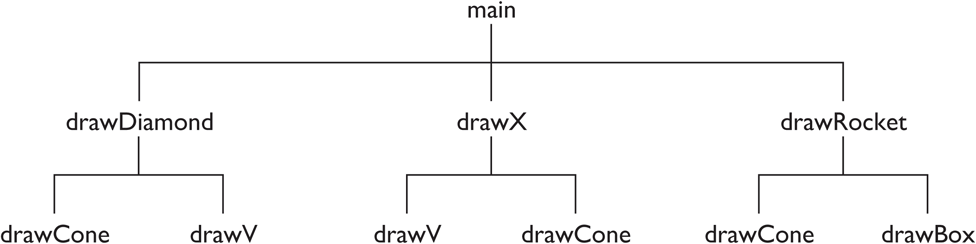
\includegraphics[width=\maxwidth,height=\maxheight,keepaspectratio,alt={Image}]{Figures/img_p95_0.png}}
\end{center}



\begin{verbatim}
 1st  main
 2nd      drawDiamond
 3rd          drawCone
 4th          drawV
 5th      drawX
 6th          drawV
 7th          drawCone
 8th      drawRocket
 9th          drawCone
10th          drawBox
11th          drawBox
12th          drawCone
\end{verbatim}

Hãy nhớ rằng thứ tự mà bạn định nghĩa các phương thức không cần phải
song song với thứ tự chúng được thực thi. Thứ tự thực thi được quyết
định bởi phần thân của phương thức \texttt{main} và bởi các phần thân
của các phương thức được gọi từ \texttt{main}. Một lời khai báo phương
thức tĩnh giống như một mục từ trong từ điển---nó định nghĩa một từ,
nhưng không xác định từ đó sẽ được sử dụng như thế nào. Phần thân của
phương thức \texttt{main} của chương trình này nói rằng hãy thực thi
\texttt{drawDiamond} trước, sau đó \texttt{drawX}, sau đó
\texttt{drawRocket}. Đây là thứ tự thực thi, bất kể thứ tự mà các phương
thức được định nghĩa.

Java cho phép bạn định nghĩa các phương thức theo bất kỳ thứ tự nào bạn
thích. Bắt đầu với \texttt{main} ở trên cùng và đi dần xuống các phương
thức ở cấp độ ngày càng thấp là một cách tiếp cận phổ biến để sử dụng,
nhưng nhiều người thích làm ngược lại, đặt các phương thức cấp thấp ở
đầu và \texttt{main} ở cuối. Java không quan tâm bạn dùng thứ tự nào,
nên bạn có thể tự quyết định và làm điều gì bạn thấy tốt nhất. Dù vậy,
sự nhất quán là quan trọng, để sau này bạn có thể dễ dàng tìm thấy một
phương thức trong một chương trình lớn.

Quan trọng là phải lưu ý rằng các chương trình \texttt{DrawFigures1},
\texttt{DrawFigures2}, và \texttt{DrawFigures3} đều tạo ra kết quả y hệt
nhau ra cửa sổ console. Tuy \texttt{DrawFigures1} có thể là chương trình
dễ đọc nhất đối với người mới bắt đầu, \texttt{DrawFigures2} và đặc biệt
là \texttt{DrawFigures3} có nhiều lợi thế hơn nó. Thứ nhất, một giải
pháp được cấu trúc tốt sẽ dễ hiểu hơn, và bản thân các phương thức trở
thành một phương tiện để giải thích chương trình. Hơn nữa, các chương
trình có các phương thức thì linh hoạt hơn và có thể dễ dàng thích ứng
với các tác vụ tương tự nhưng khác biệt. Bạn có thể lấy bảy phương thức
được định nghĩa trong \texttt{DrawFigures3} và viết một chương trình mới
để tạo ra một đầu ra lớn hơn và phức tạp hơn. Việc xây dựng các phương
thức tĩnh để tạo các lệnh mới làm tăng độ linh hoạt của bạn mà không
thêm vào sự phức tạp không cần thiết. Ví dụ, bạn có thể thay thế phương
thức \texttt{main} bằng một phiên bản gọi các phương thức khác theo thứ
tự mới sau đây. Nó sẽ tạo ra kết quả gì?

\begin{verbatim}
public static void main(String[] args) {
    drawCone();
    drawCone();
    drawRocket();
    drawX();
    drawRocket();
    drawDiamond();
    drawBox();
    drawDiamond();
    drawX();
    drawRocket();
}
\end{verbatim}

\subsection{Tóm tắt Chương (Chapter
Summary)}\label{tuxf3m-tux1eaft-chux1b0ux1a1ng-chapter-summary}

\begin{itemize}
\tightlist
\item
  Máy tính thực thi các tập hợp lệnh được gọi là chương trình
  (programs). Máy tính lưu trữ thông tin nội bộ dưới dạng chuỗi các số 0
  và số 1 (số nhị phân - binary numbers).
\item
  Ngành lập trình và khoa học máy tính xử lý các thuật toán
  (algorithms), đó là các mô tả từng bước để giải quyết vấn đề.
\item
  Java là một ngôn ngữ lập trình hướng đối tượng hiện đại được Sun
  Microsystems phát triển, nay thuộc sở hữu của Tập đoàn Oracle, ngôn
  ngữ này có một tập hợp thư viện lớn mà bạn có thể sử dụng để xây dựng
  các chương trình phức tạp.
\item
  Một chương trình được dịch từ văn bản thành các lệnh máy tính bởi một
  chương trình khác gọi là trình biên dịch (compiler). Trình biên dịch
  của Java chuyển đổi các chương trình Java thành một định dạng đặc biệt
  gọi là mã byte (Java bytecodes), mã này được thực thi bằng một chương
  trình đặc biệt gọi là Môi trường Thực thi Java (Java Runtime
  Environment).
\item
  Các lập trình viên Java thường hoàn thành công việc của mình bằng cách
  sử dụng một chương trình soạn thảo được gọi là Môi trường Phát triển
  Tích hợp (Integrated Development Environment - IDE). Các lệnh có thể
  khác nhau tùy từng môi trường, nhưng một quá trình ba bước tương tự
  luôn luôn được sử dụng:

  \begin{enumerate}
  \def\labelenumi{\arabic{enumi}.}
  \tightlist
  \item
    Nhập một chương trình dưới dạng một lớp Java (Java class).
  \item
    Biên dịch (Compile) file chương trình.
  \item
    Chạy (Run) phiên bản đã biên dịch của chương trình.
  \end{enumerate}
\item
  Java sử dụng một lệnh tên là \texttt{System.out.println} để hiển thị
  văn bản trên màn hình console.
\item
  Từ ngữ viết trong một chương trình có thể mang các ý nghĩa khác nhau.
  Từ khóa (Keywords) là các từ dành riêng đặc biệt, là một phần của ngôn
  ngữ. Định danh (Identifiers) là các từ được lập trình viên định nghĩa
  để đặt tên cho các thực thể trong chương trình. Từ cũng có thể được
  đặt vào chuỗi ký tự (strings), đó là các đoạn văn bản có thể được in
  ra console.
\item
  Các chương trình Java sử dụng khoảng trắng và bố cục hợp lý sẽ dễ đọc
  hơn đối với các lập trình viên. Tính dễ đọc cũng được nâng cao bằng
  cách viết các chú ý gọi là chú thích (comments) vào bên trong chương
  trình.
\item
  Ngôn ngữ Java có một cú pháp (syntax), hay một tập hợp các lệnh hợp lệ
  có thể được sử dụng. Một chương trình Java không tuân theo đúng cú
  pháp sẽ không biên dịch được. Một chương trình biên dịch thành công
  nhưng được viết sai vẫn có thể chứa các lỗi gọi là biệt lệ
  (exceptions) xảy ra khi chương trình chạy. Loại lỗi thứ ba là lỗi
  logic hoặc lỗi ý định (intent error). Loại lỗi này xảy ra khi chương
  trình chạy nhưng không làm được điều mà lập trình viên dự định.
\item
  Lệnh trong chương trình được gọi là các câu lệnh (statements). Một lớp
  có thể nhóm các câu lệnh thành các lệnh lớn hơn gọi là các phương thức
  tĩnh (static methods). Phương thức tĩnh giúp lập trình viên nhóm mã
  vào các phần có thể tái sử dụng. Một phương thức tĩnh quan trọng bắt
  buộc phải có trong mọi chương trình được gọi là \texttt{main}.
\item
  Nâng cấp lặp (Iterative enhancement) là quá trình xây dựng một chương
  trình từng phần một, kiểm thử chương trình ở mỗi bước trước khi tiến
  lên bước tiếp theo.
\item
  Các nhiệm vụ lập trình phức tạp nên được chia nhỏ thành các nhiệm vụ
  chính mà máy tính phải thực hiện. Quá trình này được gọi là phân rã
  thủ tục (procedural decomposition). Sử dụng đúng các phương thức tĩnh
  hỗ trợ việc phân rã thủ tục.
\end{itemize}

\subsection{Bài tập Tự kiểm tra (Self-Check
Problems)}\label{buxe0i-tux1eadp-tux1ef1-kiux1ec3m-tra-self-check-problems}

\subsubsection{Mục 1.1: Các Khái niệm Máy tính Cơ bản (Basic Computing
Concepts)}\label{mux1ee5c-1.1-cuxe1c-khuxe1i-niux1ec7m-muxe1y-tuxednh-cux1a1-bux1ea3n-basic-computing-concepts}

\begin{enumerate}
\def\labelenumi{\arabic{enumi}.}
\tightlist
\item
  Tại sao máy tính lại sử dụng số nhị phân (binary numbers)?
\item
  Chuyển đổi từng số thập phân sau đây thành số nhị phân tương đương của
  nó:

  \begin{enumerate}
  \def\labelenumii{\alph{enumii}.}
  \tightlist
  \item
    6
  \item
    44
  \item
    72
  \item
    131
  \end{enumerate}
\item
  Số thập phân tương đương của từng số nhị phân sau đây là gì?

  \begin{enumerate}
  \def\labelenumii{\alph{enumii}.}
  \tightlist
  \item
    100
  \item
    1011
  \item
    101010
  \item
    1001110
  \end{enumerate}
\item
  Bằng lời của bạn, hãy mô tả một thuật toán (algorithm) để nướng bánh
  quy. Giả sử rằng bạn có một số lượng lớn bạn bè đang đói, vì vậy bạn
  sẽ muốn tạo ra nhiều mẻ bánh quy!
\item
  Sự khác biệt giữa file \texttt{MyProgram.java} và file
  \texttt{MyProgram.class} là gì?
\end{enumerate}

\subsubsection{Mục 1.2: Và Bây giờ---Java (And
Now---Java)}\label{mux1ee5c-1.2-vuxe0-buxe2y-giux1eddjava-and-nowjava}

\begin{enumerate}
\def\labelenumi{\arabic{enumi}.}
\setcounter{enumi}{5}
\item
  Những từ nào sau đây có thể được sử dụng trong một chương trình Java
  như là các định danh (identifiers)?

\begin{verbatim}
println         first-name   AnnualSalary   "hello"   ABC
42isTheAnswer   for          sum_of_data    _average  B4
\end{verbatim}
\item
  Cú pháp nào sau đây là đúng để xuất ra một thông báo?

  \begin{enumerate}
  \def\labelenumii{\alph{enumii}.}
  \tightlist
  \item
    \texttt{System.println(Hello,\ world!);}
  \item
    \texttt{System.println.out(\textquotesingle{}Hello,\ world!\textquotesingle{});}
  \item
    \texttt{System.println("Hello,\ world!");}
  \item
    \texttt{System.out.println("Hello,\ world!");}
  \item
    \texttt{Out.system.println"(Hello,\ world!)";}
  \end{enumerate}
\item
  Đầu ra được tạo ra từ các câu lệnh sau là gì?

\begin{verbatim}
System.out.println("\"Quotes\"");
System.out.println("Slashes \\//");
System.out.println("How '\"confounding' \"\\\" it is!");
\end{verbatim}
\item
  Đầu ra được tạo ra từ các câu lệnh sau là gì?

\begin{verbatim}
System.out.println("name\tage\theight");
System.out.println("Archie\t17\t5'9\"");
System.out.println("Betty\t17\t5'6\"");
System.out.println("Jughead\t16\t6'");
\end{verbatim}
\item
  Đầu ra được tạo ra từ các câu lệnh sau là gì?

\begin{verbatim}
System.out.println("Shaq is 7'1");
System.out.println("The string \"\" is an empty message.");
System.out.println("\\'\"\"");
\end{verbatim}
\item
  Đầu ra được tạo ra từ các câu lệnh sau là gì?

\begin{verbatim}
System.out.println("\ta\tb\tc");
System.out.println("\\\\");
System.out.println("'");
System.out.println("\"\"\"");
System.out.println("C:\nin\the downward spiral");
\end{verbatim}
\item
  Đầu ra được tạo ra từ các câu lệnh sau là gì?

\begin{verbatim}
System.out.println("Dear \"DoubleSlash\" magazine,");
System.out.println();
System.out.println("\tYour publication confuses me. Is it");
System.out.println("a \\\\ slash or a //// slash?");
System.out.println("\nSincerely,");
System.out.println("Susan \"Suzy\" Smith");
\end{verbatim}
\item
  Chuỗi lệnh \texttt{println} nào sẽ tạo ra đầu ra sau đây?

\begin{verbatim}
"Several slashes are sometimes seen,"
said Sally. "I've said so." See?
\ / \\ // \\\ ///
\end{verbatim}
\item
  Chuỗi lệnh \texttt{println} nào sẽ tạo ra đầu ra sau đây?

\begin{verbatim}
This is a test of your
knowledge of "quotes" used
in 'string literals.'
You're bound to "get it right"
if you read the section on
''quotes.''
\end{verbatim}
\item
  Viết một lệnh \texttt{println} tạo ra đầu ra sau:

\begin{verbatim}
/ \ // \\ /// \\\
\end{verbatim}
\item
  Viết lại đoạn mã sau dưới dạng một chuỗi các câu lệnh
  \texttt{System.out.println} tương đương (nghĩa là không có bất kỳ lệnh
  \texttt{System.out.print} nào):

\begin{verbatim}
System.out.print("Twas ");
System.out.print("brillig and the");
System.out.println(" ");
System.out.print(" slithy toves did");
System.out.print(" ");
System.out.println("gyre and");
System.out.println("gimble");
System.out.println();
System.out.println( "in the wabe.");
\end{verbatim}
\item
  Đầu ra của chương trình sau là gì? Lưu ý rằng chương trình có chứa một
  số chú thích (comments).

\begin{verbatim}
 1  public class Commentary {
 2      public static void main(String[] args) {
 3          System.out.println("some lines of code");
 4          System.out.println("have // characters on them");
 5          System.out.println("which means ");  // that they are comments
 6          // System.out.println("written by the programmer.");
 7
 8          System.out.println("lines can also");
 9          System.out.println("have /* and */ characters");
10          /* System.out.println("which represents");
11          System.out.println("a multi-line style");
12          */ System.out.println("of comment.");
13      }
14  }
\end{verbatim}
\end{enumerate}

\subsubsection{Mục 1.3: Lỗi Chương trình (Program
Errors)}\label{mux1ee5c-1.3-lux1ed7i-chux1b0ux1a1ng-truxecnh-program-errors}

\begin{enumerate}
\def\labelenumi{\arabic{enumi}.}
\setcounter{enumi}{17}
\item
  Hãy gọi tên ba lỗi trong chương trình sau:

\begin{verbatim}
1  public MyProgram {
2      public static void main(String[] args) {
3          System.out.println("This is a test of the")
4          System.out.Println("emergency broadcast system.");
5      }
6  }
\end{verbatim}
\item
  Hãy gọi tên bốn lỗi trong chương trình sau:

\begin{verbatim}
1  public class SecretMessage {
2      public static main(string[] args) {
3          System.out.println("Speak friend");
4          System.out.println("and enter);
5
6  }
\end{verbatim}
\item
  Hãy gọi tên bốn lỗi trong chương trình sau:

\begin{verbatim}
 1  public class FamousSpeech
 2      public static void main(String[]) {
 3          System.out.println("Four score and seven years ago,");
 4          System.out.println("our fathers brought forth on");
 5          System.out.println("this continent a new nation");
 6          System.out.println("conceived in liberty,");
 7          System.out.println("and dedicated to the proposition");
 8          System.out.println("that");    /* this part should
 9          System.out.println("all");        really say,
10          System.out.println("men");        "all PEOPLE!" */
11          System.out.println("are";
12          System.out.println("created");
13          System.out.println("equal");
14      }
15  }
\end{verbatim}
\end{enumerate}

\subsection{Bài tập (Exercises)}\label{buxe0i-tux1eadp-exercises}

\begin{enumerate}
\def\labelenumi{\arabic{enumi}.}
\item
  Viết một chương trình Java hoàn chỉnh có tên \texttt{Stewie} để in ra
  kết quả sau:

\begin{verbatim}
//////////////////////
|| Victory is mine! ||
\\\\\\\\\\\\\\\\\\\\\\
\end{verbatim}
\item
  Viết một chương trình Java hoàn chỉnh có tên \texttt{Spikey} để in ra
  kết quả sau:

\begin{verbatim}
  \/
 \\//
\\\///
///\\\
 //\\
  /\
\end{verbatim}
\item
  Viết một chương trình Java hoàn chỉnh có tên \texttt{WellFormed} để in
  ra kết quả sau:

\begin{verbatim}
A well–formed Java program has
a main method with { and }
braces.

A System.out.println statement
has ( and ) and usually a
String that starts and ends
with a " character.
(But we type \" instead!)
\end{verbatim}
\item
  Viết một chương trình Java hoàn chỉnh có tên \texttt{Difference} để in
  ra kết quả sau:

\begin{verbatim}
What is the difference between
a ' and a "? Or between a " and a \"?
One is what we see when we're typing our program.
The other is what appears on the "console."
\end{verbatim}
\item
  Viết một chương trình Java hoàn chỉnh có tên \texttt{MuchBetter} để in
  ra kết quả sau:

\begin{verbatim}
A "quoted" String is
'much' better if you learn
the rules of "escape sequences."
Also, "" represents an empty String.
Don't forget: use \" instead of " !
'' is not the same as "
\end{verbatim}
\item
  Viết một chương trình Java hoàn chỉnh có tên \texttt{Meta} mà đầu ra
  của nó chính là đoạn mã nguồn của một chương trình Java in ra ``Hello,
  world!'' dưới dạng đầu ra.
\item
  Viết một chương trình Java hoàn chỉnh có tên \texttt{Mantra} để in ra
  kết quả sau. Hãy sử dụng ít nhất một phương thức tĩnh ngoài
  \texttt{main}.

\begin{verbatim}
There's one thing every coder must understand:
The System.out.println command.
There's one thing every coder must understand:
The System.out.println command.
\end{verbatim}
\item
  Viết một chương trình Java hoàn chỉnh có tên \texttt{Stewie2} để in ra
  kết quả sau. Hãy sử dụng ít nhất một phương thức tĩnh ngoài
  \texttt{main}.

\begin{verbatim}
//////////////////////
|| Victory is mine! ||
\\\\\\\\\\\\\\\\\\\\\\
|| Victory is mine! ||
\\\\\\\\\\\\\\\\\\\\\\
|| Victory is mine! ||
\\\\\\\\\\\\\\\\\\\\\\
|| Victory is mine! ||
\\\\\\\\\\\\\\\\\\\\\\
|| Victory is mine! ||
\\\\\\\\\\\\\\\\\\\\\\
\end{verbatim}
\item
  Viết một chương trình có tên \texttt{Egg} hiển thị đầu ra như sau:

\begin{verbatim}
   _______ 
  /       \ 
 /         \ 
 -"-'-"-'-"- 
 \         / 
  \_______/
\end{verbatim}
\item
  Sửa đổi chương trình từ bài tập trước để trở thành một chương trình
  mới \texttt{Egg2} hiển thị đầu ra như sau. Sử dụng các phương thức
  tĩnh sao cho phù hợp.

\begin{verbatim}
  _______
 /       \
/         \
\         /
 \_______/
-"-'-"-'-"-
  _______
 /       \
/         \
\         /
 \_______/
-"-'-"-'-"-
\         /
 \_______/
  _______
 /       \
/         \
-"-'-"-'-"-
\         /
 \_______/
\end{verbatim}
\end{enumerate}

\subsubsection{Định danh và Từ khóa (Identifiers and
Keywords)}\label{ux111ux1ecbnh-danh-vuxe0-tux1eeb-khuxf3a-identifiers-and-keywords}

Các từ được sử dụng để đặt tên cho các phần của một chương trình Java
được gọi là \textbf{định danh (identifiers)}.

\begin{quote}
\textbf{Định danh (Identifier)} Một cái tên được đặt cho một thực thể
trong một chương trình, chẳng hạn như một lớp hoặc một phương thức.
\end{quote}

Định danh phải bắt đầu bằng một chữ cái, theo sau có thể là bất kỳ số
lượng chữ cái hoặc chữ số nào. Các ví dụ sau đây đều là các định danh
hợp lệ: \texttt{first}, \texttt{hiThere}, \texttt{numStudents},
\texttt{TwoBy4}

Đặc tả ngôn ngữ Java (Java language specification) định nghĩa tập hợp
các chữ cái bao gồm cả dấu gạch dưới và ký tự đô la (\texttt{\_} và
\texttt{\$}), có nghĩa là các ví dụ sau cũng là các định danh hợp lệ:
\texttt{two\_plus\_two}, \texttt{\_count}, \texttt{\$2donuts},
\texttt{MAX\_COUNT}

Các ví dụ sau đây là các định danh không hợp lệ: \texttt{two+two},
\texttt{hi\ there}, \texttt{hi-There}, \texttt{2by4}

Java có các quy ước về việc viết hoa được các lập trình viên tuân thủ
khá nhất quán. Tất cả các tên lớp nên bắt đầu bằng một chữ cái viết hoa,
như với các lớp \texttt{Hello}, \texttt{Hello2} và \texttt{Hello3} đã
giới thiệu trước đó. Tên của các phương thức nên bắt đầu bằng chữ cái
viết thường, như trong phương thức \texttt{main}. Khi bạn ghép một số từ
lại với nhau để tạo thành một tên lớp hoặc phương thức, hãy viết hoa chữ
cái đầu tiên của mỗi từ sau từ đầu tiên. Trong chương tiếp theo, chúng
ta sẽ thảo luận về các hằng số (constants), có một quy tắc viết hoa
khác, với tất cả các chữ cái đều viết hoa và các từ được phân tách bằng
dấu gạch dưới.

Những quy tắc khác nhau này có vẻ như là những ràng buộc tẻ nhạt, nhưng
việc sử dụng viết hoa nhất quán trong mã của bạn cho phép người đọc
nhanh chóng nhận ra các phần tử mã khác nhau.

Ví dụ, giả sử bạn định ghép các từ ``all my children'' thành một định
danh. Kết quả sẽ là: - \texttt{AllMyChildren} cho một tên lớp (mỗi từ
bắt đầu bằng một chữ in hoa) - \texttt{allMyChildren} cho một tên phương
thức (bắt đầu bằng chữ in thường, các từ tiếp theo viết hoa chữ cái đầu)
- \texttt{ALL\_MY\_CHILDREN} cho tên một hằng số (tất cả viết hoa, các
từ cách nhau bằng dấu gạch dưới; được mô tả trong Chương 2)

Java phân biệt chữ hoa chữ thường (case sensitive), vì vậy các định danh
\texttt{class}, \texttt{Class}, \texttt{CLASS} và \texttt{cLASs} đều
được coi là khác nhau. Hãy ghi nhớ điều này khi bạn đọc\ldots{}

\emph{(Hình ảnh)}

các thông báo lỗi từ trình biên dịch. Con người rất giỏi trong việc hiểu
những gì bạn viết, ngay cả khi bạn viết sai chính tả các từ hoặc mắc
những sai lầm nhỏ như thay đổi chữ hoa chữ thường của một từ. Tuy nhiên,
những sai lầm như thế này khiến trình biên dịch Java trở nên vô cùng bối
rối.

Đừng ngần ngại sử dụng các định danh dài. Tên của bạn càng mang tính mô
tả (descriptive), mọi người (bao gồm cả bạn) sẽ càng dễ đọc chương trình
của bạn hơn. Các định danh có tính mô tả rất đáng để bỏ thời gian gõ. Ví
dụ, lớp \texttt{String} của Java có một phương thức tên là
\texttt{compareToIgnoreCase}.

Tuy nhiên, hãy lưu ý rằng Java có một tập hợp các định danh được xác
định trước gọi là các \textbf{từ khóa (keywords)} được dành riêng cho
các mục đích cụ thể. Trong quá trình đọc cuốn sách này, bạn sẽ học nhiều
từ khóa này và công dụng của chúng. Bạn chỉ có thể sử dụng các từ khóa
cho các mục đích đã định của chúng. Bạn phải cẩn thận tránh sử dụng
những từ này trong tên của các định danh. Ví dụ, nếu bạn đặt tên cho một
phương thức là \texttt{short} hoặc \texttt{try}, điều này sẽ gây ra vấn
đề, vì \texttt{short} và \texttt{try} là các từ khóa dành riêng. Bảng
1.4 hiển thị danh sách đầy đủ các từ khóa dành riêng.

\emph{(Bảng 1.4: Danh sách các từ khóa Java)}

\subsubsection{Một Ví dụ Phức tạp: DrawFigures1 (A Complex
Example)}\label{mux1ed9t-vuxed-dux1ee5-phux1ee9c-tux1ea1p-drawfigures1-a-complex-example}

Lệnh \texttt{println} có thể được sử dụng để vẽ các hình bằng văn bản
dưới dạng đầu ra. Hãy xem xét ví dụ chương trình phức tạp hơn sau đây
(lưu ý rằng nó sử dụng hai lệnh \texttt{println} rỗng để tạo ra các dòng
trống):

\begin{verbatim}
 1  public class DrawFigures1 {
 2      public static void main(String[] args) {
 3          System.out.println("   /\\");
 4          System.out.println("  /  \\");
 5          System.out.println(" /    \\");
 6          System.out.println(" \\    /");
 7          System.out.println("  \\  /");
 8          System.out.println("   \\/");
 9          System.out.println();
10          System.out.println(" \\    /");
11          System.out.println("  \\  /");
12          System.out.println("   \\/");
13          System.out.println("   /\\");
14          System.out.println("  /  \\");
15          System.out.println(" /    \\");
16          System.out.println();
17          System.out.println("   /\\");
18          System.out.println("  /  \\");
19          System.out.println(" /    \\");
20          System.out.println("+------+");
21          System.out.println("|      |");
22          System.out.println("|      |");
23          System.out.println("+------+");
24          System.out.println("|United|");
25          System.out.println("|States|");
26          System.out.println("+------+");
27          System.out.println("|      |");
28          System.out.println("|      |");
29          System.out.println("+------+");
30          System.out.println("   /\\");
31          System.out.println("  /  \\");
32          System.out.println(" /    \\");
33      }
34  }
\end{verbatim}

Sau đây là đầu ra mà chương trình tạo ra. Lưu ý rằng chương trình bao
gồm các ký tự gạch chéo ngược kép
(\texttt{\textbackslash{}\textbackslash{}}), nhưng đầu ra có các ký tự
gạch chéo ngược đơn. Đây là một ví dụ về \textbf{trình tự thoát (escape
sequence)}, như đã được mô tả trước đó.

\begin{verbatim}
   /\ 
  /  \ 
 /    \ 
 \    / 
  \  / 
   \/ 

 \    / 
  \  / 
   \/ 
   /\ 
  /  \ 
 /    \ 

   /\ 
  /  \ 
 /    \ 
+------+ 
|      | 
|      | 
+------+ 
|United| 
|States| 
+------+ 
|      | 
|      | 
+------+ 
   /\ 
  /  \ 
 /    \
\end{verbatim}

\subsubsection{Chú thích và Tính dễ đọc (Comments and
Readability)}\label{chuxfa-thuxedch-vuxe0-tuxednh-dux1ec5-ux111ux1ecdc-comments-and-readability}

Java là một ngôn ngữ có định dạng tự do (free-format language). Điều này
có nghĩa là bạn có thể đưa vào bao nhiêu khoảng trắng và dòng trống tùy
thích, miễn là bạn đặt ít nhất một khoảng trắng hoặc dấu câu khác giữa
các từ. Tuy nhiên, bạn nên nhớ rằng bố cục của một chương trình có thể
nâng cao (hoặc làm giảm đi) tính dễ đọc (readability) của nó. Chương
trình sau đây là hợp lệ nhưng khó đọc:

\begin{verbatim}
1  public class Ugly{public static void main(String[] args)
2  {System.out.println("How short I am!");}}
\end{verbatim}

Dưới đây là một số quy tắc đơn giản nên tuân theo sẽ làm cho chương
trình của bạn dễ đọc hơn: - Đặt các tiêu đề lớp (class headers) và
phương thức (method headers) trên các dòng riêng biệt. - Đặt không quá
một câu lệnh (statement) trên mỗi dòng. - Thụt lề chương trình của bạn
một cách hợp lý. Khi xuất hiện dấu ngoặc nhọn mở, hãy tăng mức thụt lề
của các dòng theo sau nó. Khi xuất hiện dấu ngoặc nhọn đóng, hãy giảm
lùi lề. Thụt lề các câu lệnh bên trong cặp ngoặc nhọn một khoảng trống
nhất quán (một lựa chọn phổ biến là bốn khoảng trắng cho mỗi mức thụt
lề). - Sử dụng các dòng trống để phân tách các phần của chương trình (ví
dụ: các phương thức).

Sử dụng các quy tắc này để viết lại chương trình \texttt{Ugly} mang lại
mã sau:

\begin{verbatim}
1  public class Ugly {
2      public static void main(String[] args) {
3          System.out.println("How short I am!");
4      }
5   }
\end{verbatim}

Các chương trình Java được viết tốt có thể khá dễ đọc, nhưng bạn thường
sẽ muốn đưa vào một số lời giải thích không phải là một phần của bản
thân chương trình. Bạn có thể chú thích (annotate) các chương trình bằng
cách đưa các ghi chú được gọi là \textbf{chú thích (comments)} vào trong
chúng.

\begin{quote}
\textbf{Chú thích (Comment)} Văn bản mà các lập trình viên đưa vào một
chương trình để giải thích mã code của họ. Trình biên dịch (compiler) sẽ
bỏ qua các chú thích.
\end{quote}

Có hai dạng chú thích trong Java. Ở dạng đầu tiên, bạn mở chú thích bằng
dấu gạch chéo theo sau là dấu hoa thị và đóng nó bằng dấu hoa thị theo
sau là dấu gạch chéo:

\begin{verbatim}
/* like this */
\end{verbatim}

Bạn không được đặt khoảng trắng giữa dấu gạch chéo và dấu hoa thị:

\begin{verbatim}
/ * this is bad * /
\end{verbatim}

Bạn có thể đặt hầu như bất kỳ văn bản nào bạn muốn, bao gồm nhiều dòng,
vào trong chú thích:

\begin{verbatim}
/* Thaddeus Martin
   Assignment #1
   Instructor: Professor Walingford
   Grader:     Bianca Montgomery      */
\end{verbatim}

Thứ duy nhất bạn không được phép đặt bên trong một chú thích là các ký
tự kết thúc chú thích. Mã sau đây không hợp lệ:

\begin{verbatim}
/* This comment has an asterisk/slash /*/ in it,
   which prematurely closes the comment. This is bad. */
\end{verbatim}

Java cũng cung cấp một dạng chú thích thứ hai cho các chú thích ngắn
hơn, trên một dòng (single-line comments). Bạn có thể sử dụng hai dấu
gạch chéo liên tiếp để biểu thị rằng phần còn lại của dòng hiện tại (tất
cả mọi thứ bên phải của hai dấu gạch chéo) là một chú thích. Ví dụ, bạn
có thể đặt một chú thích sau một câu lệnh:

\begin{verbatim}
System.out.println("You win!"); // Good job!
\end{verbatim}

Hoặc bạn có thể tạo một chú thích trên một dòng riêng biệt của nó:

\begin{verbatim}
// give an introduction to the user
System.out.println("Welcome to the game of blackjack.");
System.out.println();
System.out.println("Let me explain the rules.");
\end{verbatim}

Bạn thậm chí có thể tạo các khối (blocks) của các chú thích trên một
dòng:

\begin{verbatim}
// Thaddeus Martin
// Assignment #1
// Instructor:  Professor Walingford
// Grader:      Bianca Montgomery
\end{verbatim}

Một số người thích sử dụng dạng chú thích thứ nhất cho các chú thích kéo
dài nhiều dòng nhưng sử dụng dạng thứ hai an toàn hơn vì bạn không phải
nhớ đóng chú thích. Nó cũng làm cho chú thích nổi bật hơn. Đây là một
trường hợp khác mà, nếu giảng viên của bạn không yêu cầu bạn sử dụng một
kiểu chú thích cụ thể, bạn nên tự quyết định kiểu nào bạn thích hơn và
sử dụng nó nhất quán.

Đừng nhầm lẫn giữa chú thích (comments) và văn bản của các lệnh
\texttt{println}. Văn bản trong chú thích của bạn sẽ không được hiển thị
làm đầu ra khi chương trình thực thi. Chú thích chỉ ở đó để giúp người
đọc kiểm tra và hiểu chương trình.

Nên bao gồm các chú thích ở đầu mỗi file class để cho biết class đó thực
hiện chức năng gì. Bạn cũng có thể muốn cung cấp thông tin về việc bạn
là ai, bạn đang học khóa học nào, tên của giáo viên hướng dẫn hoặc người
chấm điểm của bạn, ngày tháng, v.v. Bạn cũng nên chú thích từng phương
thức để giải thích chức năng của nó.

Việc ghi chú thích trở nên hữu ích hơn trong các chương trình lớn hơn và
phức tạp hơn, cũng như trong các chương trình sẽ được xem xét hoặc sửa
đổi bởi nhiều lập trình viên. Những chú thích rõ ràng cực kỳ hữu ích để
giải thích cho người khác, hoặc cho chính bạn vào lúc khác, rằng chương
trình của bạn đang làm gì và tại sao nó làm điều đó.

Bên cạnh hai dạng chú thích đã thảo luận, Java còn hỗ trợ một kiểu chú
thích cụ thể được gọi là chú thích \textbf{Javadoc}. Định dạng của chúng
phức tạp hơn, nhưng chúng có ưu điểm là bạn có thể sử dụng một chương
trình để trích xuất các chú thích để tạo thành các file HTML có thể đọc
được bằng trình duyệt web. Chú thích Javadoc hữu ích trong lập trình
nâng cao hơn và được thảo luận chi tiết hơn trong Phụ lục B.

\emph{(Hình ảnh)}

\subsection{Lỗi chương trình (Program
Errors)}\label{lux1ed7i-chux1b0ux1a1ng-truxecnh-program-errors}

Năm 1949, Maurice Wilkes, một người tiên phong thuở đầu trong ngành máy
tính, đã bày tỏ một quan điểm mà cho đến ngày nay vẫn còn đúng:
\textgreater{} Ngay khi chúng tôi bắt đầu lập trình, chúng tôi đã ngạc
nhiên khi phát hiện ra rằng việc viết cho chương trình chạy đúng không
hề dễ dàng như chúng tôi tưởng. Quá trình gỡ lỗi (debugging) đã phải
được khám phá ra. Tôi có thể nhớ lại khoảnh khắc chính xác khi tôi nhận
ra rằng một phần lớn cuộc đời mình kể từ lúc đó trở đi sẽ là dành để tìm
ra những sai sót trong các chương trình của chính tôi.

Bạn cũng sẽ phải đối mặt với thực tế này khi bạn học lập trình. Bạn sẽ
phạm những sai lầm, giống như bất kỳ lập trình viên nào khác trong lịch
sử, và bạn sẽ cần các chiến lược để loại bỏ những sai lầm đó. Thật may
là, bản thân máy tính có thể giúp bạn làm một số phần việc.

Có ba loại lỗi bạn sẽ gặp khi bạn viết các chương trình: 1. \textbf{Lỗi
cú pháp (Syntax errors)} xảy ra khi bạn sử dụng sai ngôn ngữ Java. Chúng
tương đương với việc dùng sai ngữ pháp và bị trình biên dịch (Java
compiler) bắt lỗi. 2. \textbf{Lỗi logic (Logic errors)} xảy ra khi bạn
viết mã code không thực hiện đúng nhiệm vụ mà nó dự định phải làm. 3.
\textbf{Lỗi thời gian chạy (Runtime errors)} là những lỗi logic nghiêm
trọng đến mức Java ngăn chương trình của bạn tiếp tục thực thi.

\subsubsection{Lỗi Cú pháp (Syntax
Errors)}\label{lux1ed7i-cuxfa-phuxe1p-syntax-errors}

Con người có xu hướng khá bao dung với những sai lầm nhỏ trong lời nói.
Ví dụ, nhân vật Yoda sẽ bị trừ điểm do dùng ngữ pháp khác thường trong
bất kỳ lớp học viết nào, nhưng chúng ta vẫn hiểu ông ấy muốn nói gì.

Trình biên dịch Java sẽ kém bao dung hơn nhiều. Trình biên dịch sẽ báo
cáo các lỗi cú pháp khi nó cố gắng dịch chương trình của bạn từ Java
sang bytecodes nếu chương trình của bạn phá vỡ bất kỳ quy tắc ngữ pháp
nào của Java. Ví dụ, nếu bạn đặt sai vị trí một dấu chấm phẩy trong
chương trình của mình, bạn có thể đẩy trình biên dịch vào sự hỗn loạn
khó gỡ. Trình biên dịch có thể báo cáo một số thông báo lỗi, tùy thuộc
vào việc nó cho rằng có điều gì sai với chương trình của bạn.

Một chương trình sinh ra các lỗi biên dịch (compilation errors) thì
không thể được thực thi. Nếu bạn nộp chương trình của mình cho trình
biên dịch và trình biên dịch báo cáo lỗi, bạn phải sửa chữa lỗi và biên
dịch lại. Bạn sẽ không thể tiến xa hơn cho đến khi chương trình của bạn
không còn lỗi biên dịch.

Một số môi trường phát triển, chẳng hạn như Eclipse, trợ giúp bạn trong
suốt quá trình bằng cách gạch chân các lỗi cú pháp khi bạn viết chương
trình. Điều này giúp bạn dễ dàng phát hiện chính xác vị trí lỗi xảy ra.

Bạn có thể tự đưa ra một lỗi ngay cả trước khi bạn bắt đầu viết chương
trình, nếu bạn chọn sai tên cho file của nó.

\paragraph{LỖI LẬP TRÌNH PHỔ
BIẾN}\label{lux1ed7i-lux1eadp-truxecnh-phux1ed5-biux1ebfn}

\textbf{Tên File Không Khớp Tên Lớp (File Name Does Not Match Class
Name)} Như đã đề cập trước đó, Java yêu cầu tên lớp của một chương trình
và tên file của nó phải khớp với nhau. Ví dụ, một chương trình bắt đầu
với \texttt{public\ class\ Hello} phải được lưu trữ trong một file có
tên \texttt{Hello.java}.

Nếu bạn sử dụng sai tên file (ví dụ, lưu nó dưới tên
\texttt{WrongFileName.java}), bạn sẽ nhận được một thông báo lỗi như thế
này:

\begin{verbatim}
WrongFileName.java:1: error: class Hello is public,
    should be declared in a file named Hello.java
public class Hello {
       ^
1 error
\end{verbatim}

Tên file chỉ là rào cản đầu tiên. Có thể còn có một số lỗi khác xuất
hiện trong chương trình Java của bạn. Một trong những lỗi cú pháp phổ
biến nhất là đánh vần sai một từ (misspell a word). Bạn có thể mắc các
lỗi dấu câu, chẳng hạn như thiếu dấu chấm phẩy. Cũng dễ dàng để quên
toàn bộ một từ, chẳng hạn như một từ khóa (keyword) bắt buộc.

Thông báo lỗi mà trình biên dịch cung cấp có thể hữu ích hoặc không. Nếu
bạn không hiểu nội dung của thông báo lỗi, hãy tìm dấu mũ
(\texttt{\^{}}) bên dưới dòng lệnh, nó chỉ vào vị trí trên dòng nơi mà
trình biên dịch đã gặp rắc rối. Điều này có thể giúp bạn xác định chính
xác vị trí có thể bị thiếu một từ khóa bắt buộc.

\paragraph{LỖI LẬP TRÌNH PHỔ
BIẾN}\label{lux1ed7i-lux1eadp-truxecnh-phux1ed5-biux1ebfn-1}

\textbf{Lỗi Chính tả (Misspelled Words)} Java (cũng như hầu hết các ngôn
ngữ lập trình) rất khắt khe về lỗi chính tả. Bạn cần phải đánh vần từng
từ một cách chính xác, bao gồm cả việc viết hoa thích hợp. Ví dụ, giả sử
rằng bạn sẽ thay thế câu lệnh \texttt{println} trong chương trình
``hello world'' bằng lệnh sau:

\begin{verbatim}
System.out.pruntln("Hello, world!");
\end{verbatim}

Khi bạn thử biên dịch chương trình này, nó sẽ sinh ra một thông báo lỗi
tương tự như sau:

\begin{verbatim}
Hello.java:3: error: cannot find symbol
symbol : method pruntln(java.lang.String)
location: variable out of type PrintStream
        System.out.pruntln("Hello, world!");
                  ^
1 error
\end{verbatim}

Dòng đầu tiên của kết quả này chỉ ra rằng lỗi xảy ra trong file
\texttt{Hello.java} trên dòng số 3 và lỗi đó là trình biên dịch không
thể tìm thấy một biểu tượng (cannot find a symbol). Dòng thứ hai chỉ ra
rằng biểu tượng mà nó không tìm thấy là một phương thức có tên
\texttt{pruntln}. Đó là vì không có phương thức nào như vậy; phương thức
đó được gọi là \texttt{println}. Thông báo lỗi có thể có các dạng hơi
khác nhau tùy thuộc vào những gì bạn đã viết sai chính tả. Ví dụ, bạn có
thể quên không viết hoa từ \texttt{System}:

\begin{verbatim}
system.out.println("Hello, world!");
\end{verbatim}

Bạn sẽ nhận được thông báo lỗi sau:

\begin{verbatim}
Hello.java:3: error: package system does not exist
        system.out.println("Hello, world!");
              ^
1 error
\end{verbatim}

Một lần nữa, dòng đầu tiên cho biết lỗi xảy ra ở dòng 3 của file
\texttt{Hello.java}. Dù vậy, thông báo lỗi ở đây hơi khác, cho biết rằng
nó không thể tìm thấy gói (package) nào có tên là \texttt{system}. Dòng
thứ hai và thứ ba của thông báo lỗi này bao gồm dòng mã gốc với một mũi
tên (dấu mũ) chỉ vào nơi trình biên dịch gặp vấn đề. Lỗi của trình biên
dịch không phải lúc nào cũng rất rõ ràng, nhưng nếu bạn chú ý đến vị trí
mũi tên đang chỉ, bạn sẽ có ý tưởng khá tốt về nơi lỗi xảy ra.

Nếu bạn vẫn không thể tìm ra lỗi, hãy thử xem số dòng của lỗi và so sánh
nội dung của dòng đó với các dòng tương tự trong các chương trình khác.
Bạn cũng có thể nhờ người khác, chẳng hạn như giảng viên hoặc trợ giảng
(lab assistant), kiểm tra giúp chương trình của bạn.

\paragraph{LỖI LẬP TRÌNH PHỔ
BIẾN}\label{lux1ed7i-lux1eadp-truxecnh-phux1ed5-biux1ebfn-2}

\textbf{Quên một Dấu chấm phẩy (Forgetting a Semicolon)} Tất cả các câu
lệnh của Java đều phải kết thúc bằng các dấu chấm phẩy, nhưng bạn rất dễ
quên việc đặt một dấu chấm phẩy ở cuối câu lệnh, như trong chương trình
sau:

\begin{verbatim}
1  public class MissingSemicolon {
2      public static void main(String[] args) {
3           System.out.println("A rose by any other name")
4           System.out.println("would smell as sweet");
5      }
6  }
\end{verbatim}

Trong trường hợp này, trình biên dịch tạo ra đầu ra tương tự như sau:

\begin{verbatim}
MissingSemicolon.java:3: error: ';' expected 
        System.out.println("A rose by any other name") 
                                                     ^ 
1 error
\end{verbatim}

\paragraph{LỖI LẬP TRÌNH PHỔ
BIẾN}\label{lux1ed7i-lux1eadp-truxecnh-phux1ed5-biux1ebfn-3}

\textbf{Quên một Từ khóa Yêu cầu (Forgetting a Required Keyword)} Một
lỗi cú pháp phổ biến khác là quên một từ khóa bắt buộc khi bạn đang gõ
chương trình của mình, chẳng hạn như \texttt{static} hoặc
\texttt{class}. Hãy kiểm tra kỹ chương trình của bạn theo các ví dụ
trong sách giáo khoa để đảm bảo bạn chưa bỏ sót một từ khóa quan trọng
nào. Trình biên dịch sẽ đưa ra các thông báo lỗi khác nhau tùy thuộc vào
việc từ khóa nào bị thiếu, nhưng các thông báo có thể khó hiểu. Ví dụ,
bạn có thể viết một chương trình có tên \texttt{Bug4} và quên từ khóa
\texttt{class} khi viết tiêu đề lớp. Trong trường hợp này, trình biên
dịch sẽ đưa ra thông báo lỗi sau:

\begin{verbatim}
Bug4.java:1: error: class, interface, or enum expected
public Bug4 {
       ^
1 error
\end{verbatim}

Tuy nhiên, nếu bạn quên từ khóa \texttt{void} khi khai báo phương thức
\texttt{main}, trình biên dịch sẽ tạo ra một thông báo lỗi khác:

\begin{verbatim}
Bug5.java:2: error: invalid method declaration; return type required
    public static main(String[] args) {
                  ^
1 error
\end{verbatim}

Một lỗi cú pháp phổ biến khác là quên đóng chuỗi ký tự bằng dấu nháy.
Một nguyên tắc kinh nghiệm hữu ích để làm theo là: lỗi đầu tiên được
trình biên dịch báo cáo là lỗi quan trọng nhất. Các lỗi còn lại có thể
là hậu quả của lỗi đầu tiên đó. Nhiều lập trình viên thậm chí không buồn
quan tâm đến các lỗi phía sau lỗi đầu tiên, bởi vì việc sửa lỗi đầu tiên
và biên dịch lại có thể khiến các lỗi kia biến mất.

\subsubsection{Lỗi logic (Logic Errors hay
Bugs)}\label{lux1ed7i-logic-logic-errors-hay-bugs}

Lỗi logic còn được gọi là rệp (bugs). Các lập trình viên máy tính dùng
các từ như ``đầy rệp'' (bug-ridden) và ``có rệp'' (buggy) để mô tả những
chương trình viết tệ, và quá trình tìm và loại bỏ rệp khỏi các chương
trình được gọi là \textbf{gỡ lỗi (debugging)}.

Từ ``bug'' là một thuật ngữ kỹ thuật cổ xưa có từ trước khi máy tính
xuất hiện; những con ``rệp'' thời kỳ đầu máy tính đôi khi xuất hiện ở cả
phần cứng cũng như phần mềm. Đô đốc Grace Hopper, một người tiên phong
trong ngành máy tính, được coi là người đã phổ biến rộng rãi việc sử
dụng thuật ngữ này trong bối cảnh lập trình máy tính. Bà thường kể lại
một câu chuyện có thật về nhóm các lập trình viên ở trường Đại học
Harvard vào giữa những năm 1940, những người không thể hiểu được chương
trình của mình bị lỗi ở đâu cho tới khi họ mở chiếc máy tính ra và phát
hiện có một con bướm đêm (moth) thật bị mắc kẹt bên trong.

Hình thức của một con bệp có thể đa dạng. Đôi khi, chương trình của bạn
chỉ đơn giản là cư xử không đúng đắn. Ví dụ, nó có thể tạo ra đầu ra
sai. Vào những lúc khác, nó sẽ yêu cầu máy tính thực hiện một nhiệm vụ
rõ ràng là một sự nhầm lẫn, trong trường hợp này, chương trình của bạn
sẽ gặp lỗi thời gian chạy (runtime error) khiến nó phải ngừng thực thi.
Trong chương này, do kiến thức Java của bạn còn hạn chế, nhìn chung loại
lỗi logic duy nhất mà bạn sẽ gặp phải là một sai lầm trong đầu ra của
chương trình do sử dụng câu lệnh \texttt{println} hay lệnh gọi hàm
(method call) không chính xác.

Chúng ta sẽ xem xét một ví dụ về lỗi thời gian chạy ở phần tiếp theo.

\subsection{Phân rã Thủ tục (Procedural
Decomposition)}\label{phuxe2n-ruxe3-thux1ee7-tux1ee5c-procedural-decomposition}

Brian Kernighan, đồng tác giả của cuốn \emph{The C Programming
Language}, đã nói, ``Kiểm soát sự phức tạp là bản chất của lập trình máy
tính.'' Con người chỉ có một khả năng khiêm tốn đối với các chi tiết.
Chúng ta không thể giải quyết những vấn đề phức tạp cùng một lúc. Thay
vào đó, chúng ta cấu trúc việc giải quyết vấn đề của mình bằng cách chia
nhỏ vấn đề thành các phần có thể quản lý được và chinh phục từng phần
một. Chúng ta thường sử dụng thuật ngữ \textbf{phân rã (decomposition)}
để mô tả nguyên tắc này khi áp dụng vào lập trình.

\begin{quote}
\textbf{Phân rã (Decomposition)} Sự chia tách thành các phần có thể nhận
biết được, trong đó mỗi phần đơn giản hơn toàn thể.
\end{quote}

Với các ngôn ngữ lập trình thủ tục (procedural programming languages)
như C, việc phân rã liên quan đến việc chia một nhiệm vụ phức tạp thành
một tập hợp các nhiệm vụ con. Đây là một cách tiếp cận mang định hướng
động từ hoặc hành động rất cao, bao gồm việc chia nhỏ hành động tổng thể
thành một loạt các hành động nhỏ hơn. Kỹ thuật này được gọi là
\textbf{phân rã thủ tục (procedural decomposition)}.

\paragraph{LỖI LẬP TRÌNH PHỔ
BIẾN}\label{lux1ed7i-lux1eadp-truxecnh-phux1ed5-biux1ebfn-4}

\textbf{Không Đóng Chuỗi Ký tự hoặc Chú thích (Not Closing a String
Literal or Comment)} Mỗi chuỗi ký tự phải có một dấu ngoặc kép mở và một
dấu ngoặc kép đóng, nhưng rất dễ quên dấu ngoặc kép đóng. Ví dụ, bạn có
thể viết:

\begin{verbatim}
System.out.println("Hello, world!);
\end{verbatim}

Điều này tạo ra ba thông báo lỗi khác nhau, mặc dù chỉ có một lỗi cú
pháp cơ bản:

\begin{verbatim}
Hello.java:3: error: unclosed string literal
        System.out.println("hello world);
                     ^
Hello.java:3: error: ';' expected
        System.out.println("hello world);
                            ^
Hello.java:5: error: reached end of file while parsing
    }
    ^
3 errors
\end{verbatim}

Trong trường hợp này, thông báo lỗi đầu tiên khá rõ ràng, bao gồm một
mũi tên chỉ vào phần đầu của chuỗi ký tự chưa được đóng. Thông báo lỗi
thứ hai là do nguyên nhân từ lỗi thứ nhất. Vì chuỗi ký tự không được
đóng, trình biên dịch đã không nhận ra dấu ngoặc đơn đóng và dấu chấm
phẩy xuất hiện ở cuối dòng.

Một vấn đề tương tự xảy ra khi bạn quên đóng một chú thích nhiều dòng
bằng cách viết \texttt{*/}, như trong dòng đầu tiên của chương trình
sau:

\begin{verbatim}
/* This is a bad program.
public class Bad {
   public static void main(String[] args){
       System.out.println("Hi there.");
  }
} /* end of program */
\end{verbatim}

File trên không phải là một chương trình; nó là một chú thích dài. Vì
chú thích ở dòng đầu tiên không được đóng, nên toàn bộ chương trình đã
bị nuốt chửng. May mắn thay, nhiều chương trình soạn thảo Java (Java
editor programs) tô màu các phần của một chương trình để giúp bạn nhận
biết chúng bằng mắt thường. Thông thường, nếu bạn quên đóng một chuỗi ký
tự hoặc chú thích, phần còn lại của chương trình của bạn sẽ chuyển sang
màu sai, điều này có thể giúp bạn phát hiện ra lỗi.

Java được thiết kế cho một loại phân rã khác mang định hướng danh từ
hoặc đối tượng (object-oriented) nhiều hơn. Thay vì coi vấn đề như một
loạt các hành động cần thực hiện, chúng ta coi nó như một tập hợp các
đối tượng (objects) phải tương tác với nhau.

Là một nhà khoa học máy tính, bạn nên quen thuộc với cả hai kiểu giải
quyết vấn đề. Cuốn sách này bắt đầu với phân rã thủ tục và dành nhiều
chương để làm chủ các khía cạnh khác nhau của phương pháp tiếp cận thủ
tục. Chỉ sau khi bạn đã thực hành nhuần nhuyễn lập trình thủ tục, chúng
ta mới chuyển sự chú ý trở lại phân rã đối tượng và lập trình hướng đối
tượng.

Như một ví dụ về phân rã thủ tục, hãy xem xét vấn đề nướng một chiếc
bánh (baking a cake). Bạn có thể chia vấn đề này thành các vấn đề con
(subproblems) sau: - Làm bột (Make the batter). - Nướng bánh (Bake the
cake). - Làm kem phủ (Make the frosting). - Phủ kem lên bánh (Frost the
cake).

Mỗi một trong bốn nhiệm vụ này có các chi tiết đi kèm với nó. Ví dụ, để
làm bột, bạn làm theo các bước sau: - Trộn các nguyên liệu khô (Mix the
dry ingredients). - Đánh bông bơ và đường (Cream the butter and sugar).
- Đánh trứng vào (Beat in the eggs). - Khuấy nguyên liệu khô vào (Stir
in the dry ingredients).

Như vậy, bạn chia nhiệm vụ tổng thể thành các nhiệm vụ con, mà bạn lại
tiếp tục chia thành các nhiệm vụ con nhỏ hơn nữa. Cuối cùng, bạn đạt đến
các mô tả đơn giản đến mức không cần giải thích thêm (tức là, các phép
toán nguyên thủy - primitives).

Một sơ đồ một phần của quá trình phân rã này được hiển thị trong Hình
1.2. ``Make cake'' là thao tác ở mức cao nhất. Nó được định nghĩa dựa
trên bốn thao tác ở mức thấp hơn gọi là ``Make batter,'' ``Bake,''
``Make frosting,'' và ``Frost cake.'' Thao tác ``Make batter'' lại được
định nghĩa dựa trên các thao tác ở mức thậm chí thấp hơn nữa, và điều
tương tự có thể được thực hiện cho ba thao tác kia. Sơ đồ này được gọi
là một \textbf{sơ đồ cấu trúc (structure diagram)} và nhằm mục đích chỉ
ra cách một vấn đề được phân tách thành các vấn đề con. Trong sơ đồ này,
bạn cũng có thể biết các thao tác được thực hiện theo thứ tự nào bằng
cách đọc từ trái sang phải. Điều đó không đúng đối với hầu hết các sơ đồ
cấu trúc. Để xác định thứ tự thực tế mà các chương trình con được thực
hiện, bạn thường phải tham chiếu đến bản thân chương trình.

\emph{(Hình 1.2: Phân rã nhiệm vụ ``Make cake'')}

\begin{figure}
\centering


\begin{center}
\pandocbounded{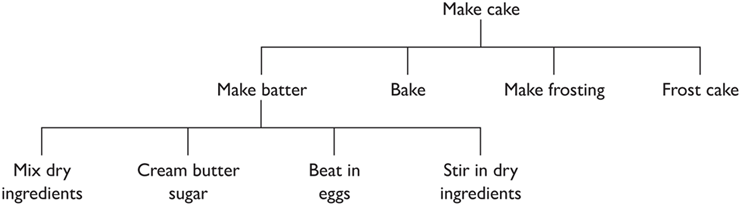
\includegraphics[width=\maxwidth,height=\maxheight,keepaspectratio,alt={Image}]{Figures/img_p65_1.png}}
\end{center}


\caption{Image}
\end{figure}

Một thuật ngữ giải quyết vấn đề cuối cùng liên quan đến quá trình lập
trình. Các lập trình viên chuyên nghiệp phát triển các chương trình theo
từng giai đoạn. Thay vì cố gắng tạo ra một chương trình hoàn chỉnh chạy
được cùng một lúc, họ chọn một phần của vấn đề để cài đặt trước. Sau đó
họ thêm một phần khác, và một phần khác, và một phần khác nữa. Tổng thể
chương trình được xây dựng lên một cách từ từ, từng mảnh một. Quá trình
này được gọi là \textbf{nâng cấp lặp (iterative enhancement)} hoặc
\textbf{tinh chỉnh từng bước (stepwise refinement)}.

\begin{quote}
\textbf{Nâng cấp lặp (Iterative Enhancement)} Quá trình tạo ra một
chương trình theo từng giai đoạn, bổ sung chức năng mới ở mỗi giai đoạn.
Một tính năng quan trọng của mỗi bước lặp là bạn có thể kiểm thử (test)
nó để đảm bảo phần đó hoạt động tốt trước khi chuyển sang bước tiếp
theo.
\end{quote}

Bây giờ, chúng ta hãy xem xét một cấu trúc sẽ cho phép bạn nâng cấp lặp
các chương trình Java của mình để cải thiện cấu trúc của chúng và giảm
bớt sự dư thừa (redundancy): các phương thức tĩnh (static methods).

\subsubsection{Các Phương thức Tĩnh (Static
Methods)}\label{cuxe1c-phux1b0ux1a1ng-thux1ee9c-tux129nh-static-methods}

Java được thiết kế cho các đối tượng (objects), và lập trình trong Java
thường liên quan đến việc phân rã một vấn đề thành các đối tượng khác
nhau, mỗi đối tượng có các phương thức thực hiện những nhiệm vụ cụ thể.
Bạn sẽ thấy cách điều này hoạt động trong các chương sau, nhưng bây giờ,
chúng bản phân rã thủ tục. Chúng ta sẽ hoãn việc xem xét một số chi tiết
của Java lại trong khi chúng ta thảo luận về lập trình nói chung.

Hãy xem xét chương trình sau, vẽ hai hộp văn bản trên cửa sổ console:

\begin{verbatim}
 1  // This program draws two box figures.
 2  public class DrawBoxes {
 3       public static void main(String[] args) {
 4           System.out.println("+------+");
 5           System.out.println("|      |");
 6           System.out.println("|      |");
 7           System.out.println("+------+");
 8           System.out.println();
 9           System.out.println("+------+");
10           System.out.println("|      |");
11           System.out.println("|      |");
12           System.out.println("+------+");
13       }
14   }
\end{verbatim}

\emph{(Hình ảnh minh họa)}

Chương trình hoạt động chính xác, nhưng bốn dòng được dùng để vẽ hộp
xuất hiện hai lần. Sự lặp lại (redundancy) này là không mong muốn vì một
số lý do. Ví dụ, bạn có thể muốn thay đổi hình thức của các hộp, trong
trường hợp đó bạn sẽ phải thực hiện mọi chỉnh sửa hai lần. Ngoài ra, bạn
có thể muốn vẽ thêm các hộp khác, điều này sẽ yêu cầu bạn phải gõ thêm
các bản sao (hoặc copy và paste) các dòng trùng lặp.

Chúng ta có thể cải thiện chương trình bằng cách giới thiệu một lệnh mới
để vẽ cái hộp và sau đó thực thi lệnh đó hai lần. Java không có một lệnh
``vẽ một cái hộp'', nhưng bạn có thể tạo ra một lệnh như vậy. Một lệnh
được đặt tên như vậy được gọi là một \textbf{phương thức tĩnh (static
method)}.

\begin{quote}
\textbf{Phương thức Tĩnh (Static Method)} Một khối (block) các câu lệnh
Java được đặt cho một cái tên.
\end{quote}

Các phương thức tĩnh là các đơn vị của quá trình phân rã thủ tục. Chúng
ta thường chia một lớp (class) thành một vài phương thức tĩnh, mỗi
phương thức giải quyết một phần nào đó của vấn đề tổng thể. Ví dụ, đây
là một phương thức tĩnh để vẽ một cái hộp:

\begin{verbatim}
public static void drawBox() {
    System.out.println("+------+");
    System.out.println("|      |");
    System.out.println("|      |");
    System.out.println("+------+");
}
\end{verbatim}

Bạn đã nhìn thấy một phương thức tĩnh có tên là \texttt{main} trong các
chương trình trước đó. Nhớ lại rằng phương thức \texttt{main} có dạng
sau:

\begin{verbatim}
public static void main(String[] args) {
    <statement>;
    <statement>;
    ...
    <statement>;
}
\end{verbatim}

Các phương thức tĩnh mà bạn sẽ viết có cấu trúc tương tự:

\begin{verbatim}
public static void <name>() {
    <statement>;
    <statement>;
    ...
    <statement>;
}
\end{verbatim}

Dòng đầu tiên được gọi là \textbf{tiêu đề phương thức (method header)}.
Bạn chưa cần phải hiểu đầy đủ ý nghĩa của từng phần trong tiêu đề này
trong Java; hiện tại, chỉ cần nhớ rằng bạn sẽ cần viết
\texttt{public\ static\ void}, theo sau là tên mà bạn muốn đặt cho
phương thức, theo sau là một cặp dấu ngoặc đơn. Nói ngắn gọn, đây là ý
nghĩa của các từ trong tiêu đề: - Từ khóa \texttt{public} cho biết
phương thức này có sẵn để được sử dụng bởi tất cả các phần trong chương
trình của bạn. Mọi phương thức bạn viết sẽ đều là \texttt{public}. - Từ
khóa \texttt{static} cho biết đây là một phương thức tĩnh (theo phong
cách thủ tục, không phải hướng đối tượng). Hiện tại, mọi phương thức bạn
viết sẽ là \texttt{static}, cho đến khi bạn học về định nghĩa đối tượng
trong Chương 8. - Từ khóa \texttt{void} cho biết phương thức này thực
thi các câu lệnh nhưng không tạo ra (trả về) bất kỳ giá trị nào. (Các
phương thức khác mà bạn sẽ thấy sau này tính toán và trả về các giá
trị.) - \texttt{\textless{}name\textgreater{}} (ví dụ: \texttt{drawBox})
là tên của phương thức. - Cặp ngoặc đơn trống xác định một danh sách
(trong trường hợp này, một danh sách trống) các giá trị được gửi tới
phương thức của bạn như là đầu vào; các giá trị như vậy được gọi là
\textbf{tham số (parameters)} và sẽ không được đưa vào các phương thức
của bạn cho đến Chương 3.

Việc bao gồm từ khóa \texttt{static} cho mỗi phương thức bạn định nghĩa
có vẻ cồng kềnh. Các sách giáo khoa Java khác thường không thảo luận về
các phương thức tĩnh sớm như chúng tôi làm ở đây; thay vào đó, họ chỉ ra
các kỹ thuật khác để phân rã vấn đề. Nhưng mặc dù các phương thức tĩnh
cần một chút công sức để tạo ra, chúng là những công cụ mạnh mẽ và hữu
ích để cải thiện các chương trình Java cơ bản.

\emph{(Hình ảnh)}

Sau phần tiêu đề trong phương thức mẫu của chúng ta, một chuỗi các lệnh
\texttt{println} tạo nên \textbf{phần thân (body)} của phương thức tĩnh
này. Giống như trong phương thức \texttt{main}, các câu lệnh của phương
thức này được thực thi theo thứ tự từ đầu đến cuối.

Bằng cách định nghĩa phương thức \texttt{drawBox}, bạn đã gán một cái
tên đơn giản cho chuỗi lệnh \texttt{println} này. Nó giống như việc nói
với trình biên dịch Java, ``Bất cứ khi nào tôi bảo bạn `drawBox', ý tôi
thực sự là bạn nên thực thi các câu lệnh \texttt{println} trong phương
thức \texttt{drawBox}.'' Nhưng lệnh sẽ không thực sự được thực thi trừ
khi phương thức \texttt{main} của chúng ta trình bày rõ ràng
(explicitly) rằng nó muốn làm vậy. Hành động thực thi một phương thức
tĩnh được gọi là \textbf{lời gọi hàm (method call)}.

\begin{quote}
\textbf{Lời gọi Hàm (Method Call)} Một lệnh để thực thi một phương thức
khác, điều này làm cho tất cả các câu lệnh bên trong phương thức đó được
thực thi.
\end{quote}

Để thực thi lệnh \texttt{drawBox}, hãy đưa dòng này vào phương thức
\texttt{main} của chương trình của bạn:

\begin{verbatim}
drawBox();
\end{verbatim}

Do chúng ta muốn thực thi lệnh \texttt{drawBox} hai lần (để vẽ hai hộp),
phương thức \texttt{main} nên chứa hai lời gọi đến phương thức
\texttt{drawBox}. Chương trình sau sử dụng phương thức \texttt{drawBox}
để tạo ra đầu ra giống như chương trình \texttt{DrawBoxes} ban đầu:

\begin{verbatim}
 1  // Draws two box figures using a static method.
 2  public class DrawBoxes2 {
 3      public static void main(String[] args) {
 4          drawBox();
 5          System.out.println();
 6          drawBox();
 7      }
 8
 9      public static void drawBox() {
10          System.out.println("+------+");
11          System.out.println("|      |");
12          System.out.println("|      |");
13          System.out.println("+------+");
14      }
15  }
\end{verbatim}

\subsubsection{Luồng Điều khiển (Flow of
Control)}\label{luux1ed3ng-ux111iux1ec1u-khiux1ec3n-flow-of-control}

Điều khó hiểu nhất về các phương thức tĩnh là các chương trình chứa các
phương thức tĩnh không thực thi tuần tự từ trên xuống dưới. Thay vào đó,
mỗi khi chương trình bắt gặp một lời gọi phương thức tĩnh, việc thực thi
của chương trình ``nhảy'' đến phương thức tĩnh đó, thực thi từng câu
lệnh trong phương thức đó theo thứ tự, và sau đó ``nhảy'' trở lại điểm
bắt đầu của lời gọi và tiếp tục thực thi. Thứ tự mà các câu lệnh của một
chương trình được thực thi được gọi là \textbf{luồng điều khiển (flow of
control)} của chương trình.

\begin{quote}
\textbf{Luồng Điều khiển (Flow of Control)} Thứ tự mà các câu lệnh của
một chương trình Java được thực thi.
\end{quote}

Hãy xem xét luồng điều khiển của chương trình \texttt{DrawBoxes2} hiển
thị trước đó. Nó có hai phương thức. Phương thức đầu tiên là phương thức
quen thuộc \texttt{main}, và phương thức thứ hai là \texttt{drawBox}.
Giống như bất kỳ chương trình Java nào, quá trình thực thi bắt đầu bằng
phương thức \texttt{main}:

\begin{verbatim}
public static void main(String[] args) {
    drawBox();
    System.out.println();
    drawBox();
}
\end{verbatim}

Về một khía cạnh nào đó, quá trình thực thi chương trình này là tuần tự:
Mỗi câu lệnh được liệt kê trong phương thức \texttt{main} được thực thi
lần lượt, từ đầu đến cuối.

Nhưng phương thức \texttt{main} này bao gồm hai lời gọi khác nhau tới
phương thức \texttt{drawBox}. Chương trình này sẽ làm ba việc khác nhau:
thực thi \texttt{drawBox}, thực thi một lệnh \texttt{println}, sau đó
lại thực thi \texttt{drawBox} một lần nữa.

Sơ đồ dưới đây chỉ ra luồng điều khiển do chương trình này sinh ra.

Theo dõi sơ đồ, bạn có thể thấy rằng chín câu lệnh \texttt{println} đã
được thực thi. Đầu tiên bạn chuyển quyền điều khiển cho phương thức
\texttt{drawBox} và thực thi bốn câu lệnh của nó. Sau đó bạn quay trở
lại \texttt{main} và thực thi câu lệnh \texttt{println} của nó. Sau đó
bạn chuyển quyền điều khiển lần thứ hai tới \texttt{drawBox} và một lần
nữa thực thi bốn câu lệnh của nó.

\emph{(Sơ đồ luồng điều khiển)}


\begin{center}
\pandocbounded{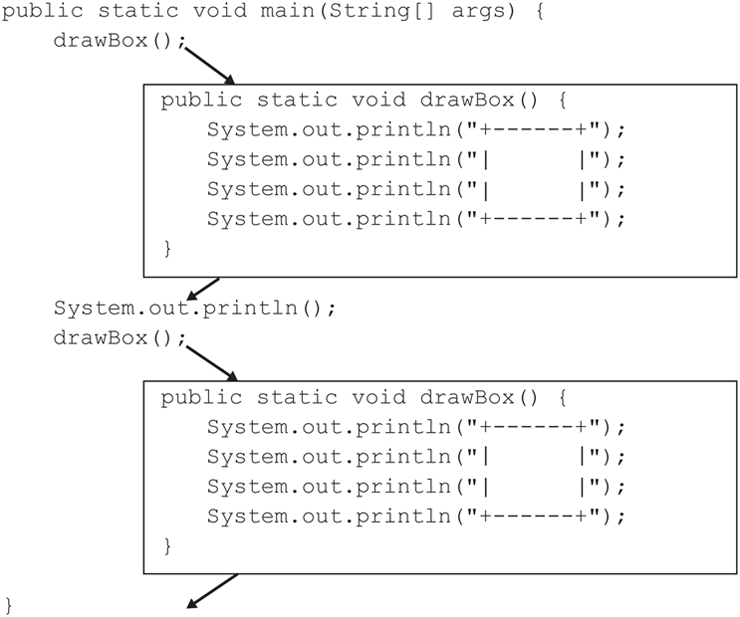
\includegraphics[width=\maxwidth,height=\maxheight,keepaspectratio,alt={Image}]{Figures/img_p75_0.png}}
\end{center}



Việc tạo ra các lời gọi hàm (method calls) này gần giống như sao chép
(copy) và dán (paste) mã của phương thức đó vào trong phương thức
\texttt{main}. Kết quả là, chương trình này có hành vi giống hệt như
phương thức \texttt{main} chín dòng của chương trình \texttt{DrawBoxes}:

\begin{verbatim}
public static void main(String[] args) {
     System.out.println("+------+");
     System.out.println("|      |");
     System.out.println("|      |");
     System.out.println("+------+");
     System.out.println();
     System.out.println("+------+");
     System.out.println("|      |");
     System.out.println("|      |");
     System.out.println("+------+");
}
\end{verbatim}

Phiên bản này đơn giản hơn về mặt luồng điều khiển của nó, nhưng phiên
bản trước tránh được sự lặp lại của việc để cùng một các lệnh
\texttt{println} xuất hiện nhiều lần. Nó cũng mang lại cảm nhận tốt hơn
về cấu trúc của giải pháp. Trong phiên bản gốc, rõ ràng là có một nhiệm
vụ con (subtask) tên là \texttt{drawBox} đang được thực hiện hai lần.
Ngoài ra, mặc dù phiên bản cuối cùng của phương thức \texttt{main} chứa
ít dòng mã hơn chương trình \texttt{DrawBoxes2}, hãy xem xét điều gì sẽ
xảy ra nếu bạn muốn thêm một hộp thứ ba vào đầu ra. Bạn sẽ phải thêm lại
năm lệnh \texttt{println} bắt buộc, trong khi ở các chương trình sử dụng
phương thức \texttt{drawBox}, bạn có thể chỉ cần thêm một lệnh
\texttt{println} nữa và một lời gọi hàm thứ ba.

Java cho phép bạn định nghĩa các phương thức theo bất kỳ thứ tự nào bạn
thích. Có một quy ước phổ biến là đặt phương thức \texttt{main} làm
phương thức đầu tiên hoặc cuối cùng trong lớp (class). Trong cuốn sách
giáo khoa này, chúng tôi thường sẽ đặt \texttt{main} đầu tiên, nhưng các
chương trình sẽ hoạt động tương tự nếu chúng ta đổi chỗ thứ tự. Ví dụ,
chương trình sửa đổi sau đây có hành vi giống hệt như chương trình
\texttt{DrawBoxes2} trước đó:

\begin{verbatim}
 1  // Draws two box figures using a static method.
 2  public class DrawBoxes3 {
 3      public static void drawBox() {
 4          System.out.println("+------+");
 5          System.out.println("|      |");
 6          System.out.println("|      |");
 7          System.out.println("+------+");
 8      }
 9
10      public static void main(String[] args) {
11          drawBox();
12          System.out.println();
13          drawBox();
14      }
15  }
\end{verbatim}

Phương thức \texttt{main} luôn là điểm bắt đầu cho việc thực thi chương
trình, và từ điểm bắt đầu đó, bạn có thể xác định thứ tự mà các phương
thức khác được gọi.

\subsubsection{Các Phương thức Gọi Các Phương thức Khác (Methods That
Call Other
Methods)}\label{cuxe1c-phux1b0ux1a1ng-thux1ee9c-gux1ecdi-cuxe1c-phux1b0ux1a1ng-thux1ee9c-khuxe1c-methods-that-call-other-methods}

Phương thức \texttt{main} không phải là nơi duy nhất bạn có thể gọi một
phương thức khác. Thực tế, bất kỳ phương thức nào cũng có thể gọi bất kỳ
phương thức nào khác. Do đó, luồng điều khiển có thể trở nên khá phức
tạp. Chẳng hạn, hãy xem xét chương trình khá kỳ lạ sau đây. Chúng tôi
chủ đích sử dụng các từ vô nghĩa (``foo,'' ``bar,'' ``baz,'' và
``mumble'') bởi vì chương trình không nhằm mục đích có ý nghĩa.

\begin{verbatim}
 1  public class FooBarBazMumble {
 2      public static void main(String[] args) {
 3          foo();
 4          bar();
 5          System.out.println("mumble");
 6      }
 7
 8      public static void foo() {
 9          System.out.println("foo");
10      }
11
12      public static void bar() {
13          baz();
14          System.out.println("bar");
15      }
16
17      public static void baz() {
18          System.out.println("baz");
19      }
20  }
\end{verbatim}

Bạn khó có thể biết dễ dàng đầu ra mà chương trình này tạo ra, vì vậy
hãy cùng khám phá chi tiết những gì chương trình đang làm. Hãy nhớ rằng
Java luôn bắt đầu với phương thức được gọi là \texttt{main}. Trong
chương trình này, phương thức \texttt{main} gọi phương thức \texttt{foo}
và phương thức \texttt{bar}, sau đó thực thi một lệnh \texttt{println}:

\begin{verbatim}
public static void main(String[] args) {
    foo();
    bar();
    System.out.println("mumble");
}
\end{verbatim}

Mỗi một trong hai lời gọi phương thức này sẽ mở rộng ra thành nhiều câu
lệnh hơn. Hãy xem xét việc mở rộng các lời gọi đến các phương thức
\texttt{foo} và \texttt{bar} trước: Điều này giúp bức tranh về luồng
điều khiển của chúng ta trở nên hoàn chỉnh hơn, nhưng hãy lưu ý rằng
\texttt{bar} lại gọi phương thức \texttt{baz}, vì vậy chúng ta cũng phải
mở rộng phương thức đó nữa.

\emph{(Hình ảnh)}


\begin{center}
\pandocbounded{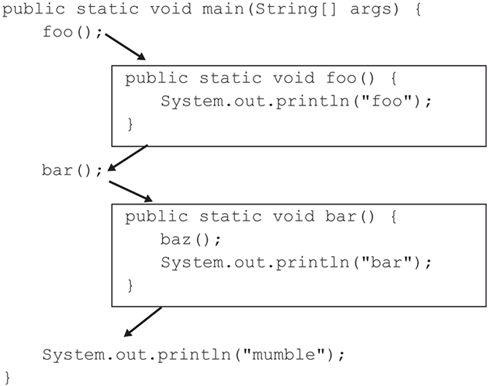
\includegraphics[width=\maxwidth,height=\maxheight,keepaspectratio,alt={Image}]{Figures/img_p80_0.png}}
\end{center}


